% !TeX root = ../../Book3.tex
% 纲要标题：## 第16章　热核、谱渐近与几何系数
% 纲要位置：几何学计划纲要.md，第 2747 行。
% 正文状态：初稿；尚未正式审核。

% 纲要内容开始
% 
% > 本章目标与证明范围：谱展开构造和短时局部参数构造分别证明，再比较二者。Weyl 渐近和逆谱问题在明确的余项与 Tauber 型输入之后展开。
% 
% 纲要内容结束

\chapter{热核、谱渐近与几何系数}
\label{g3:ch:16}
\BookChapterNumber{g3:ch:16}

\begin{chapterabstract}
	热演化把 Laplace 的离散谱与流形的局部几何放在同一个核中。本章先由谱展开及 Sobolev 估计构造光滑热核，证明半群律、最大值、质量保持和热迹公式；再在测地坐标中解运输方程，通过截断与 Volterra 修正建立带统一余项的短时展开。对角首项给出体积，下一项给出标量曲率积分。经过正测度的 Tauber 引理，热迹首项转化为 Weyl 特征值渐近。最后用变分原理建立曲率与直径估计，算出球面和环面的谱，并以两个十六维平坦环面说明完整谱仍不能确定等距类型。
\end{chapterabstract}

\begin{learninggoals}
	\begin{itemize}
		\item 从非负 Laplace 的特征展开构造热半群，证明平滑作用及 \(L^2\) 连续分布解的唯一性。
		\item 用取值泛函的平方和估计建立核级数的光滑收敛与热迹公式。
		\item 在测地坐标中求出 Gaussian 修正系数，控制截断误差及 Volterra 级数。
		\item 从法坐标体积密度计算前两个对角热系数，说明积分余项的统一性。
		\item 证明从热迹首项到谱计数首项的 Tauber 引理，并核对 Weyl 常数及尺度。
		\item 运用极小极大原则和 Bochner 公式估计特征值，识别曲率、连通性与直径的作用。
		\item 计算球面、平坦环面的特征值及重数，验证等谱不等距的具体格构造。
	\end{itemize}
\end{learninggoals}

在周长 \(2\pi\) 的圆周上，初始温度中的 \(\cos(k\theta)\) 随时间变为 \(e^{-k^2t}\cos(k\theta)\)。振荡越快，衰减越快；充分长时间以后，只剩平均温度。反过来看很短的时间，满足 \(k^2t\) 不大的频率还没有受到很强的抑制，其数量约为 \(t^{-1/2}\)。这提示我们：把所有衰减因子相加，可能从短时间行为读出高频谱的分布。

\ProseParagraphBreak

同一过程也可以从空间看。热量起初集中在一点附近，随后向周围扩散；欧氏模型中的扩散宽度是 \(\sqrt t\)。在流形上，足够小的邻域接近切空间，首先出现的仍是 Gaussian 核，但体积密度与曲率会修正它。谱展开是整体的，测地坐标计算是局部的；证明二者构造出同一个热核，便把短时几何计算变成谱的陈述。

\ProseParagraphBreak

这条联系也提出了逆向问题。若已知所有特征值及重数，能否恢复流形？本章先明确能够恢复的量，再直接构造等谱不等距的环面。例子中的格有不同的最短向量关系，却在每个长度上有相同的向量数；因此“频率及其重数”与“频率方向之间的关系”是两种不同的信息。

\ProseParagraphBreak

本章主干在光滑闭流形上展开，沿用 \(\Delta=-\operatorname{div}\operatorname{grad}\) 及正体积密度。所需分析是第十一章的 Sobolev 嵌入、第十二至十三章的椭圆正则性与离散谱；曲率系数使用第三章的法坐标展开，谱下界使用第十五章的 Bochner 公式。热核构造及迹的延伸阅读见 Berline、Getzler、Vergne 的第2.3—2.6节\cite[第2章，2.3--2.6节]{BerlineGetzlerVergne2004}；等谱环面的原始例子见 Milnor 的论文\cite[第542页]{Milnor1964Isospectral}。

% !TeX root = ../../Book3.tex
% 纲要标题：### 16.1 热半群和谱构造
% 纲要位置：几何学计划纲要.md，第 2751 行。
% 正文状态：初稿；尚未正式审核。

% 纲要内容开始
% 
% * Laplace 算子的热半群
% * 热方程解与平滑作用
% * 核的存在、对称性和半群律
% * 最大值与质量保持
% 
% 纲要内容结束

\section{热半群和谱构造}
\label{g3:sec:1601}

一个特征函数的热演化特别简单：若 \(\Delta\phi=\lambda\phi\)，则 \(e^{-t\lambda}\phi\) 满足 \(\partial_tu+\Delta u=0\)。一般初值可以按特征函数展开，因此热方程先变成各个频率独立衰减的问题。要从这个想法得到可用的热核，还须证明三件事：级数确实定义了解，正时间消除了初值的不光滑性，并且解能写成对初值的积分。本节用第十三章的谱范数及第十一章的嵌入完成这些步骤。

\subsection{Laplace 算子的热半群}
\label{g3:subsec:1601:01}

本章的基本对象是非空的 \(n\ge1\) 维光滑闭黎曼流形 \((M,g)\)，这里“闭”表示紧且无边界，不要求可定向。积分使用正体积密度 \(\mu_g\)，复 \(L^2\) 内积对第一变量线性。函数 Laplace 为
\[
	\Delta=-\operatorname{div}\operatorname{grad},\qquad
	(\Delta f,f)_{L^2}=\|\mathrm df\|_2^2\quad(f\in C^\infty(M)).
\]
由\cref{g3:thm:positive-elliptic-realization,g3:thm:elliptic-discrete-spectrum}，其定义域为 \(H^2(M)\) 的实现非负自伴，并有光滑正交归一特征基。本章从 \(0\) 开始编号，按重数排列为
\begin{equation}\label{g3:eq:heat-spectrum-enumeration}
	\Delta\phi_j=\lambda_j\phi_j,\qquad
	0=\lambda_0\le\lambda_1\le\cdots\longrightarrow\infty,
	\qquad j=0,1,\ldots.
\end{equation}
零特征函数在每个连通分支上为常数，因为其外微分的平方积分为零。紧流形只有有限多个连通分支，所以零特征值的重数就是分支数；仅当 \(M\) 连通时才有 \(\lambda_1>0\)。由于 \(\Delta\) 保持实函数，每个特征空间可选实正交基，再复化得到所需基。以下核公式允许使用任意复正交基。

\begin{definition}\label{g3:def:heat-semigroup}
	设 \((M,g)\) 为非空的正维光滑闭黎曼流形。对 \(t\ge0\) 及 \(f\in L^2(M)\)，定义
	\begin{equation}\label{g3:eq:heat-semigroup-series}
		T_tf=e^{-t\Delta}f\coloneqq
		\sum_{j=0}^{\infty}e^{-t\lambda_j}(f,\phi_j)_{L^2}\phi_j.
	\end{equation}
	这个算子族称为 \(\Delta\) 的\term[rebanqun]{热半群}[heat semigroup]。
\end{definition}

因为 \(0<e^{-t\lambda_j}\le1\)，级数在 \(L^2\) 中收敛。同一特征空间上的乘数是一个标量，换正交基不改变算子，因此定义只依赖于 \(\Delta\)。这里的指数由谱展开定义，并不要求把无界算子的幂级数逐项作用于任意 \(L^2\) 函数。

\begin{proposition}\label{g3:prop:heat-semigroup-properties}
	设 \((M,g)\) 为非空的正维光滑闭黎曼流形。上述 \(T_t\) 是自伴的 \(L^2\) 压缩算子，且
	\[
		T_0=I,\qquad T_{t+s}=T_tT_s\quad(t,s\ge0),\qquad
		T_tf\longrightarrow f\text{ 在 }L^2\text{ 中 }(t\downarrow0).
	\]
	在 \(f\in H^2(M)\) 时，\(\frac{\mathrm d}{\mathrm dt}T_tf=-\Delta T_tf\)，导数在 \(t=0\) 按右导数理解。反之，若 \((T_tf-f)/t\) 在 \(L^2\) 中有极限，则 \(f\in H^2(M)\)。
\end{proposition}
\begin{proof}
	正交展开给出 \(\|T_tf\|_2^2=\sum_j e^{-2t\lambda_j}|(f,\phi_j)|^2\le\|f\|_2^2\)，实乘数给出自伴性，乘数相乘给出半群律。由于 \(|e^{-t\lambda_j}-1|\le1\)，对平方可和的系数列使用支配收敛，得到强连续性；半群律又把这一结论移到任意时间。

	若 \(f\in H^2\)，由式\eqref{g3:eq:spectral-domain}有 \(\sum_j\lambda_j^2|(f,\phi_j)|^2<\infty\)。不等式 \(|(e^{-t\lambda}-1)/t|\le\lambda\) 允许在 \(L^2\) 中对级数求右导数，得到 \(-\Delta f\)；正时间的导数同理。反之，若差商收敛于 \(h\)，逐项与 \(\phi_j\) 配对便得 \((h,\phi_j)=-\lambda_j(f,\phi_j)\)。平方和恒等式给出上述带权可和性，故 \(f\in H^2\)。
\end{proof}

\subsection{热方程解与平滑作用}
\label{g3:subsec:1601:02}

指数衰减比任意多项式增长都快，而第十三章已将导数范数转成特征系数上的多项式权。这两件事合在一起，便能解释热方程为何立即使初值光滑。此时还不需要知道第 \(j\) 个特征值究竟增长多快。

\begin{theorem}\label{g3:thm:heat-spectral-solution}
	设 \((M,g)\) 为非空的正维光滑闭黎曼流形，\(f\in L^2(M)\)。则 \(u(t)=T_tf\) 属于 \(C([0,\infty);L^2(M))\)，在 \((0,\infty)\times M\) 上光滑，满足
	\[
		\partial_tu+\Delta u=0,\qquad u(0)=f.
	\]
	它是具有上述 \(L^2\) 连续性和初值的唯一分布解。对每个整数 \(m,p\ge0\)，存在常数 \(C_{m,p}\)，使
	\begin{equation}\label{g3:eq:heat-sobolev-smoothing}
		\|\partial_t^pT_tf\|_{H^{2m}}
		\le C_{m,p}t^{-m-p}\|f\|_2,
		\qquad 0<t\le1.
	\end{equation}
	若 \(f\) 光滑，则解及其任意阶空间、时间导数连续延伸至 \(t=0\)。
\end{theorem}
\begin{proof}
	由\cref{g3:thm:elliptic-spectral-sobolev}，\(H^{2m}\) 范数等价于系数的权 \((1+\lambda_j)^{2m}\) 的平方和。对 \(0<t\le1\)，令 \(s=t\lambda\)，则
	\[
		(1+\lambda)^m\lambda^p e^{-t\lambda}
		\le t^{-m-p}(1+s)^{m+p}e^{-s}
		\le C_{m,p}t^{-m-p}.
	\]
	这给出式\eqref{g3:eq:heat-sobolev-smoothing}。在时间区间 \([\varepsilon,A]\subset(0,\infty)\) 上，给各项乘任意次 \(\lambda_j\) 后，所有 \(H^{2m}\) 级数仍一致收敛；可先在有限和上求导，再用同一估计控制尾项。选择 \(2m>r+n/2\)，由\cref{g3:cor:higher-sobolev-embedding}得到任意 \(C^r\) 空间范数中的收敛与时间可微性。因此解联合光滑，并满足热方程。强初值已由上一命题证明。

	再设 \(v\in C([0,A];L^2)\) 为同初值的分布解。取测试函数 \(\eta(t)\overline{\phi_j(x)}\)，其中 \(\eta\in C_c^\infty((0,A))\)，便知连续函数 \(v_j(t)=(v(t),\phi_j)\) 在分布意义下满足
	\(v_j'+\lambda_jv_j=0\)。乘 \(e^{t\lambda_j}\) 后导数为零，故它为常数：一维分布导数为零的结论可由局部卷积得到，再以重叠区间上的常数相容延拓。初值确定 \(v_j(t)=e^{-t\lambda_j}(f,\phi_j)\)，完备特征基遂给出 \(v=T_tf\)。

	若 \(f\) 光滑，则其全部谱权平方和有限。对任意 \(m,p\)，对 \(\lambda_j^p(f,\phi_j)\) 使用带权支配收敛，得 \(\partial_t^pT_tf\to(-\Delta)^pf\) 在 \(H^{2m}\) 中收敛；高阶嵌入完成最后的断言。
\end{proof}

\begin{example}\label{g3:exm:circle-heat-decay}
	在周长 \(2\pi\) 的圆周上，初值 \(f(\theta)=2+\cos\theta+3\sin(4\theta)\) 演化为
	\[
		T_tf=2+e^{-t}\cos\theta+3e^{-16t}\sin(4\theta).
	\]
	平均值保持不变，四倍频率的衰减率是原来的十六倍。对于一般 \(L^2\) 初值，逐频率相乘给出的仍是同一个解；刚才的定理负责保证无穷叠加在正时间成为光滑函数。
\end{example}

能量恒等式进一步说明这种衰减的方向。对 \(t>0\)，有
\begin{equation}\label{g3:eq:heat-energy-dissipation}
	\frac{\mathrm d}{\mathrm dt}\|T_tf\|_2^2
	=-2(\Delta T_tf,T_tf)=-2\|\mathrm dT_tf\|_2^2.
\end{equation}
先在 \([\varepsilon,A]\) 上积分，再令 \(\varepsilon\downarrow0\)，得到 \(\|T_Af\|_2^2+2\int_0^A\|\mathrm dT_tf\|_2^2\,\mathrm dt=\|f\|_2^2\)。初值可以没有弱一阶导数，但正时间导数能量的这一时间积分仍有限。

\subsection{核的存在、对称性和半群律}
\label{g3:subsec:1601:03}

算子作用于整个初值函数，积分核则记录从一点到另一点的传播。把式\eqref{g3:eq:heat-semigroup-series}中的内积展开，候选核应为 \(\sum_j e^{-t\lambda_j}\phi_j(x)\overline{\phi_j(y)}\)。问题是该级数能否逐点乃至逐阶求导。以下先估计热演化后在一点取值的线性泛函，从而直接控制核级数的平方和。

\begin{lemma}\label{g3:lem:heat-evaluation-square-sum}
	设 \((M,g)\) 为非空的正维光滑闭黎曼流形。固定有限坐标覆盖，在较小坐标闭集内，对每个多重指标 \(\alpha\) 和 \(\tau>0\)，有一致估计
	\[
		\sum_{j=0}^\infty e^{-2\tau\lambda_j}
		|\partial^\alpha\phi_j(x)|^2\le C_{\alpha,\tau}.
	\]
	常数可在 \(\tau\) 的任意紧正时间区间内统一选择。
\end{lemma}
\begin{proof}
	由式\eqref{g3:eq:heat-sobolev-smoothing}及高阶嵌入，\(f\mapsto\partial^\alpha T_\tau f(x)\) 是 \(L^2\) 上的连续线性泛函，其范数一致不超过 \(C\)。在任意有限和 \(f=\sum_{j=0}^N c_j\phi_j\) 上，它等于 \(\sum_{j=0}^N c_j e^{-\tau\lambda_j}\partial^\alpha\phi_j(x)\)。在 \(\sum|c_j|^2=1\) 下取上确界，得到该有限系数列的平方和不超过 \(C^2\)。令 \(N\to\infty\) 即得结论。
\end{proof}

\begin{theorem}\label{g3:thm:heat-kernel-spectral}
	设 \((M,g)\) 为非空的正维光滑闭黎曼流形。存在唯一的光滑函数 \(K\) 定义于 \((0,\infty)\times M\times M\)，使对任意 \(f\in L^2(M)\) 有
	\begin{equation}\label{g3:eq:heat-kernel-action}
		T_tf(x)=\int_M K(t,x,y)f(y)\,\mu_g(y).
	\end{equation}
	它由级数
	\begin{equation}\label{g3:eq:heat-kernel-series}
		K(t,x,y)=\sum_{j=0}^\infty e^{-t\lambda_j}
		\phi_j(x)\overline{\phi_j(y)}
	\end{equation}
	给出；任意阶空间与时间导数在 \([\varepsilon,A]\times M\times M\) 上一致收敛，其中 \(0<\varepsilon<A<\infty\)。它为实值，满足
	\begin{align}
		K(t,x,y)&=K(t,y,x),\label{g3:eq:heat-kernel-symmetry}\\
		K(t+s,x,y)&=\int_M K(t,x,z)K(s,z,y)\,\mu_g(z)
		\quad(t,s>0),\label{g3:eq:heat-kernel-semigroup}\\
		(\partial_t+\Delta_x)K&=0.
	\end{align}
	此函数称为 \((M,g)\) 的\term[rehe]{热核}[heat kernel]。
\end{theorem}
\begin{proof}
	固定 \(\varepsilon>0\)，取任意空间导数 \(\partial_x^\alpha,\partial_y^\beta\) 和时间导数阶数 \(p\)。对 \(t\ge\varepsilon\) 及 \(j>N\)，有
	\[
		\lambda_j^p e^{-t\lambda_j}
		\le C_{p,\varepsilon}e^{-\varepsilon\lambda_{N+1}/4}
		e^{-\varepsilon\lambda_j/2}.
	\]
	因此导数级数的绝对值尾和不超过
	\[
		C_{p,\varepsilon}e^{-\varepsilon\lambda_{N+1}/4}
		\left(\sum_{j>N}e^{-\varepsilon\lambda_j/2}
		|\partial^\alpha\phi_j(x)|^2\right)^{1/2}
		\left(\sum_{j>N}e^{-\varepsilon\lambda_j/2}
		|\partial^\beta\phi_j(y)|^2\right)^{1/2}.
	\]
	上一引理以 \(\tau=\varepsilon/4\) 控制两个平方和，而前面的指数趋于零。于是级数及任意导数局部一致收敛，定义光滑核并允许逐项代入热方程。这一证明只用 \(\lambda_j\to\infty\)，并未预设计数函数的增长率。

	对有限特征和，式\eqref{g3:eq:heat-kernel-action}由正交性成立。对一般 \(f\in L^2\)，有限和在 \(L^2\) 中逼近，左侧经 \(T_t:L^2\to C^0\) 连续，右侧因连续核的各行有一致有界的 \(L^2\) 范数而连续，故积分公式仍成立。若两个连续核给出同一算子，则固定 \(x\) 后其差与所有 \(L^2\) 函数积分为零；取差的复共轭作测试，知该行恒为零，得到唯一性。

	交换 \(x,y\) 对级数取复共轭，得到 Hermitian 对称性。选实特征基时每项为实数，所以核实值，得到式\eqref{g3:eq:heat-kernel-symmetry}。半群律的两边分别是 \(T_{t+s}\) 与 \(T_tT_s\) 的连续核；积分可由紧性及核连续性交换次序，唯一性给出式\eqref{g3:eq:heat-kernel-semigroup}。
\end{proof}

\begin{proposition}\label{g3:prop:heat-kernel-trace}
	设 \((M,g)\) 为非空的正维光滑闭黎曼流形。对每个 \(t>0\)，\(T_t\) 是迹类算子，其热迹为
	\begin{equation}\label{g3:eq:heat-kernel-trace}
		Z(t)\coloneqq\operatorname{Tr}(T_t)
		=\sum_{j=0}^\infty e^{-t\lambda_j}
		=\int_M K(t,x,x)\,\mu_g(x)<\infty.
	\end{equation}
\end{proposition}
\begin{proof}
	对正紧算子，特征值之和有限即称为迹类，该和就是迹。这里 \(T_t\) 的有限谱截断在算子范数中收敛，因为尾部乘数的上确界趋于零，所以它紧且正。上一引理取 \(\alpha=0,\tau=t/2\)，给出对角级数的一致上界；各项非负，积分与求和可由单调收敛交换，得到
	\[
		\int_M\sum_j e^{-t\lambda_j}|\phi_j(x)|^2\,\mu_g(x)
		=\sum_j e^{-t\lambda_j}\|\phi_j\|_2^2.
	\]
	左侧因 \(M\) 紧而有限，正是核在对角上的积分。这个迹与所选正交基无关：任意另一正交基 \((\psi_k)\) 都满足
	\(\sum_k(T_t\psi_k,\psi_k)=\sum_{k,j}e^{-t\lambda_j}|(\psi_k,\phi_j)|^2=\sum_j e^{-t\lambda_j}\)，交换非负求和并使用完备性即可。
\end{proof}

同一构造也适用于丛值问题。若 \(E\to M\) 为正秩 Hermitian 丛，\(P\) 是光滑、形式自伴、非负的二阶椭圆算子，则把上述特征函数换成特征截面，得到光滑的 \(\operatorname{Hom}(E_y,E_x)\) 值核
\begin{equation}\label{g3:eq:bundle-heat-kernel}
	K_P(t,x,y)v=\sum_j e^{-t\lambda_j}\phi_j(x)
	\langle v,\phi_j(y)\rangle_{E_y}.
\end{equation}
有限平凡化中对各分量应用同一取值泛函估计，即可逐项得到核级数及全部导数的收敛；对称性变为 \(K_P(t,x,y)=K_P(t,y,x)^*\)，半群公式中的乘法为纤维映射复合。积分对角上的纤维迹给出 \(\operatorname{Tr}(e^{-tP})\)。因此 Hodge Laplace 及后续平方型算子也有这一谱构造；下面的标量次序结论则依赖于函数具有大小次序。

\subsection{最大值与质量保持}
\label{g3:subsec:1601:04}

对于实温度，热方程还有谱表达不直接显出的性质：最高温度不会上升，最低温度不会下降。闭流形没有边界通量，因而总热量保持不变。这些事实将使核成为一个带质量一的非负平均权。

\begin{proposition}\label{g3:prop:heat-maximum-mass}
	设 \((M,g)\) 为非空的正维光滑闭黎曼流形。其标量热核满足
	\[
		K(t,x,y)\ge0,\qquad
		\int_MK(t,x,y)\,\mu_g(y)=1
		\quad(t>0,x\in M).
	\]
	对实连续初值 \(f\)，有 \(\min_M f\le T_tf\le\max_M f\)，且 \(T_tf\to f\) 一致成立。对每个 \(1\le p\le\infty\)，核公式定义 \(L^p\) 压缩算子；对 \(p<\infty\) 它在 \(t=0\) 强连续。对任意 \(f\in L^1(M)\)，有 \(\int_MT_tf\,\mu_g=\int_Mf\,\mu_g\)。
\end{proposition}
\begin{proof}
	先设 \(f\) 为实光滑函数，\(u=T_tf\)。固定 \(A>0\) 和 \(\varepsilon>0\)，令 \(w=u-\varepsilon t\)。若 \(w\) 在 \([0,A]\times M\) 的最大值严格大于 \(\max f\)，最大点 \((t_0,x_0)\) 必有 \(t_0>0\)。在空间最大点处 \(\Delta w\ge0\)，而 \(\partial_tw(t_0,x_0)\ge0\)：内部时间点导数为零，末端时间点从左侧看导数非负。于是 \((\partial_t+\Delta)w\ge0\)，与其等于 \(-\varepsilon\) 矛盾。令 \(\varepsilon\downarrow0\) 得上界，对 \(-u\) 同理得下界。取实特征基也可见实初值保持实值。

	若在某处 \(K(t,x,y_0)<0\)，连续性给出一个 \(y_0\) 的邻域，核在其中为负。选择支撑于该邻域的非零非负光滑初值，积分公式便与刚才的非负性矛盾，故 \(K\ge0\)。由于 \(\Delta1=0\)，谱定义给出 \(T_t1=1\)，即核的行质量为一；对称性又给出列质量为一。

	非负质量一的积分权给出 \(|T_tf(x)|^p\le\int K(t,x,y)|f(y)|^p\,\mu_g(y)\)（\(1\le p<\infty\)），再按 \(x\) 积分即得 \(L^p\) 压缩性；\(p=\infty\) 直接估计积分。这也把算子延拓到全部 \(L^p\)，并由非负积分或绝对可积性保证公式合法。光滑函数在 \(C^0\) 中一致稠密，且对光滑初值已有 \(T_tf\to f\) 一致成立，利用压缩性即可逼近连续初值。对 \(p<\infty\) 使用 \(C^\infty\) 在 \(L^p\) 中稠密，得到强连续性。最后对 \(L^1\) 初值交换积分，并使用核的列质量一，得到总质量保持。
\end{proof}

\begin{proposition}\label{g3:prop:heat-large-time}
	设 \((M,g)\) 为非空的正维光滑闭黎曼流形，\(\Pi_0\) 是投影到在各连通分支上为常数的函数空间，\(\lambda_+\) 是最小正特征值。则对 \(f\in L^2(M)\)，有
	\[
		\|T_tf-\Pi_0f\|_2\le e^{-\lambda_+t}\|f-\Pi_0f\|_2.
	\]
	对每个整数 \(r\ge0\)，在 \(t\ge1\) 时还有
	\[
		\|T_tf-\Pi_0f\|_{C^r}
		\le C_r e^{-\lambda_+(t-1)}\|f-\Pi_0f\|_2.
	\]
	在一个连通分支 \(M_a\) 上，\(\Pi_0f=\operatorname{Vol}(M_a)^{-1}\int_{M_a}f\,\mu_g\)。
\end{proposition}
\begin{proof}
	去掉零特征项后，所有乘数都不超过 \(e^{-\lambda_+t}\)，平方求和得到第一式。对 \(t\ge1\) 写成 \(T_1T_{t-1}(f-\Pi_0f)\)，先用第一式，再用固定正时间的 \(L^2\to C^r\) 平滑估计，得到第二式。各分支的归一化常数函数构成零特征空间的正交基，所以投影就是逐分支平均。
\end{proof}

热核兼有两种尺度：长时间只留下每个连通分支上的平均，短时间则集中在对角附近。下一节将直接从局部度量构造短时核，并解释曲率如何进入这种集中。
% 纲要条目排为编号小节标题，并进入目录与书签；说明段仍保留于纲要注释中。

% !TeX root = ../../Book3.tex
% 纲要标题：### 16.2 短时热核的局部构造
% 纲要位置：几何学计划纲要.md，第 2758 行。
% 正文状态：初稿；尚未正式审核。

% 纲要内容开始
% 
% * 测地距离和 Gaussian 主项
% * 运输方程与系数递推
% * 截断参数核的误差
% * Volterra 修正及余项控制
% * 局部构造与谱核的一致性
% 
% 纲要内容结束

\section{短时热核的局部构造}
\label{g3:sec:1602}

热核在时间很小时主要集中于距离约为 \(\sqrt t\) 的范围。这个尺度上，切空间中的 Gaussian 核给出主项，度量及其导数则进入逐阶修正。本节从这些局部数据构造一个近似核，再用收敛的时间卷积级数消去误差。最后借上一节的唯一性识别所得核，并证明可逐阶求导的统一余项。

\subsection{测地距离和 Gaussian 主项}
\label{g3:subsec:1602:01}
本节先固定非空、\(n\ge1\) 维的光滑闭黎曼流形 \((M,g)\)，采用 \(\Delta=-\operatorname{div}\operatorname{grad}\) 和体积密度 \(\mu_g\)。流形可以不连通；下面的局部核在不同连通分支之间取零。对各连通分支使用\cref{g3:lem:uniform-normal-neighborhood}，再以紧性取统一半径，存在 \(\rho>0\)，使 \(d(x,y)<\rho\) 时可唯一写成
\[
	x=\exp_yv,\qquad v\in\mathrm T_yM,\qquad |v|=r=d(x,y).
\]
映射 \((y,v)\mapsto(\exp_yv,y)\) 在此邻域为微分同胚。用 \(\mathrm T_yM\) 上由 \(g_y\) 决定的 Euclid 密度 \(\mathrm dv\) 定义
\begin{equation}\label{g3:eq:heat-normal-density}
	\exp_y^*\mu_g=J_y(v)\,\mathrm dv,
	\qquad J(x,y)=J_y(v).
\end{equation}
于是 \(J>0\) 联合光滑，\(J(y,y)=1\)，且法坐标的一阶导数消失给出 \(\mathrm d_vJ_y(0)=0\)。这里不要求可定向。

\ProseParagraphBreak

在 Euclid 空间中，基本核为
\[
	G_{\mathbb R^n}(t,v)=(4\pi t)^{-n/2}
	\exp\!\left(-\frac{|v|^2}{4t}\right).
\]
直接求导可验证 \((\partial_t-\sum_i\partial_i^2)G_{\mathbb R^n}=0\)；逐坐标积分和一维 Gaussian 积分给出总质量为一。令 \(v=\sqrt t\,w\)，便见质量集中于 \(|v|\) 为 \(\sqrt t\) 量级的区域。因此在法邻域中取
\begin{equation}\label{g3:eq:heat-geodesic-gaussian}
	G(t,x,y)=(4\pi t)^{-n/2}e^{-r^2/(4t)}.
\end{equation}
它的指数已经使用了真实测地距离，但体积扩张还会使它偏离热方程。

\begin{figure}[htbp]
	\centering
	% !TeX root = ../Book3.tex
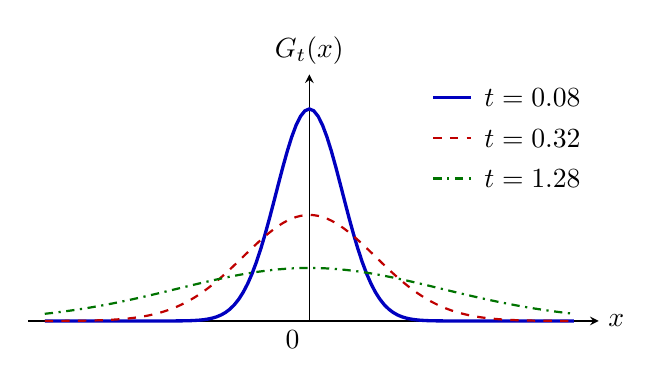
\begin{tikzpicture}[x=1.05cm,y=2.7cm,>=stealth]
	\draw[->] (-3.4,0)--(3.5,0) node[right] {\(x\)};
	\draw[->] (0,0)--(0,1.16) node[above] {\(G_t(x)\)};
	\draw[very thick,blue!75!black,domain=-3.2:3.2,samples=121]
		plot (\x,{exp(-\x*\x/.32)/sqrt(4*pi*.08)});
	\draw[thick,red!75!black,dashed,domain=-3.2:3.2,samples=121]
		plot (\x,{exp(-\x*\x/1.28)/sqrt(4*pi*.32)});
	\draw[thick,green!45!black,dash dot,domain=-3.2:3.2,samples=121]
		plot (\x,{exp(-\x*\x/5.12)/sqrt(4*pi*1.28)});
	\draw[very thick,blue!75!black] (1.5,1.05)--(1.95,1.05);
	\node[right] at (2,1.05) {\(t=0.08\)};
	\draw[thick,red!75!black,dashed] (1.5,.86)--(1.95,.86);
	\node[right] at (2,.86) {\(t=0.32\)};
	\draw[thick,green!45!black,dash dot] (1.5,.67)--(1.95,.67);
	\node[right] at (2,.67) {\(t=1.28\)};
	\node[below left] at (0,0) {\(0\)};
\end{tikzpicture}

	\caption{一维 Euclid Gaussian 核的高度与扩散尺度}
	\label{g3:fig:gaussian-scale}
\end{figure}

\Cref{g3:fig:gaussian-scale}画出三个时刻的一维模型。时间缩小为原来的四分之一时，峰值增大为两倍，集中宽度缩小为一半，而总积分仍为一。流形上将保留这种局部尺度，并用系数修正密度与曲率造成的差别。

\begin{lemma}\label{g3:lem:heat-gaussian-transport-identity}
	设 \((M^n,g)\) 为非空、\(n\ge1\) 维的光滑闭黎曼流形。在 \(d(x,y)<\rho\) 的统一法邻域中，令 \(J\) 和 \(G\) 分别由式\eqref{g3:eq:heat-normal-density}及式\eqref{g3:eq:heat-geodesic-gaussian}定义。取 \(\Delta=-\operatorname{div}\operatorname{grad}\)，定义作用于 \(x\) 变量的算子
	\[
		\mathcal T=r\partial_r+\tfrac12r\partial_r\log J.
	\]
	其中 \(r\partial_r\) 在法坐标中为 \(v^i\partial_{v^i}\)，故在对角上光滑延伸。对任意光滑的 \(a(t,x,y)\)，有
	\begin{equation}\label{g3:eq:heat-gaussian-transport-identity}
		(\partial_t+\Delta_x)(Ga)
		=G\left(\partial_ta+\Delta_xa+t^{-1}\mathcal Ta\right).
	\end{equation}
\end{lemma}
\begin{proof}
	Gauss 引理给出 \(|\mathrm d_xr|=1\)。极坐标中的体积密度为 \(r^{n-1}J_y(r\theta)\,\mathrm dr\,\mathrm d\theta\)，所以在 \(r>0\) 处
	\[
		\Delta r=-\frac{n-1}{r}-\partial_r\log J,
		\qquad \Delta(r^2)=-2n-2r\partial_r\log J.
	\]
	利用 \(\Delta(e^h)=e^h(\Delta h-|\mathrm dh|^2)\)，可得
	\[
		\frac{\partial_tG}{G}=-\frac n{2t}+\frac{r^2}{4t^2},
		\qquad
		\frac{\Delta_xG}{G}=\frac n{2t}
		+\frac{r\partial_r\log J}{2t}-\frac{r^2}{4t^2}.
	\]
	两式的 \(t^{-2}\) 项及常数 \(t^{-1}\) 项抵消。再用
	\(\Delta(Ga)=G\Delta a+a\Delta G-2\langle\mathrm dG,\mathrm da\rangle\)
	和 \(\mathrm dG/G=-r\,\mathrm dr/(2t)\)，便得结论。两边在 \(r=0\) 处均光滑，故等式也在那里成立。
\end{proof}

因而主项的修正首先是一个沿径向测地线的一阶问题。二阶算子 \(\Delta_x\) 将在后一阶才进入递推；这使系数能够逐个确定。

\subsection{运输方程与系数递推}
\label{g3:subsec:1602:02}
寻找形式为 \(G\sum_{j=0}^Nt^ju_j(x,y)\) 的近似解。代入式\eqref{g3:eq:heat-gaussian-transport-identity}，依次令 \(t^{-1},t^0,\ldots,t^{N-1}\) 的系数为零，得到\term[yunshu fangcheng]{运输方程}[transport equation]
\begin{equation}\label{g3:eq:heat-transport-recursion}
	\mathcal Tu_0=0,\qquad
	(\mathcal T+j)u_j=-\Delta_xu_{j-1}\quad(j\ge1),
	\qquad u_0(y,y)=1.
\end{equation}
最后一个条件保证对角上的质量归一化。
\symidx{\(u_j(x,y)\)：短时热核的运输系数}

\begin{proposition}\label{g3:prop:heat-transport-coefficients}
	设 \((M^n,g)\) 为非空、\(n\ge1\) 维的光滑闭黎曼流形，\(\Delta=-\operatorname{div}\operatorname{grad}\)，\(J\) 为式\eqref{g3:eq:heat-normal-density}的法坐标密度。在统一法邻域 \(d(x,y)<\rho\) 上，式\eqref{g3:eq:heat-transport-recursion}有唯一的光滑系数列。具体地，若 \(x=\exp_yv\)、\(z_s=\exp_y(sv)\)，则
	\begin{align}
		u_0(x,y)&=J_y(v)^{-1/2},\label{g3:eq:heat-u0-density}\\
		u_j(x,y)&=-J_y(v)^{-1/2}
		\int_0^1s^{j-1}J_y(sv)^{1/2}
		(\Delta_xu_{j-1})(z_s,y)\,\mathrm ds,
		\quad j\ge1.\label{g3:eq:heat-transport-integral}
	\end{align}
	特别地，
	\begin{equation}\label{g3:eq:heat-diagonal-recursion}
		u_0(y,y)=1,\qquad
		u_j(y,y)=-\frac1j(\Delta_xu_{j-1})(y,y).
	\end{equation}
\end{proposition}
\begin{proof}
	固定 \(y\) 和单位方向 \(\theta\)。把方程乘以 \(r^{j-1}J_y(r\theta)^{1/2}\)，便得到
	\[
		\partial_r\bigl(r^jJ_y(r\theta)^{1/2}u_j(\exp_y(r\theta),y)\bigr)
		=-r^{j-1}J_y(r\theta)^{1/2}
		(\Delta_xu_{j-1})(\exp_y(r\theta),y).
	\]
	当 \(j=0\) 时，右边取零，归一化给出 \(J^{1/2}u_0=1\)。当 \(j\ge1\) 时，光滑性迫使左边括号在 \(r=0\) 为零。从零积分到 \(r\)，再令积分变量为 \(rs\)，即得式\eqref{g3:eq:heat-transport-integral}。

	该积分式也证明了对角处的光滑性。若 \(u_{j-1}\) 联合光滑，其被积函数在 \((s,y,v)\in[0,1]\times\{|v|<\rho\}\) 上光滑，任意固定阶导数可移入有限区间积分，因而 \(u_j\) 联合光滑。由归纳得到全部系数。齐次方程的差解满足 \(r^jJ^{1/2}w\) 沿径向恒定；\(j\ge1\) 时光滑性使该常数为零，\(j=0\) 时由归一化也为零。这证明唯一性。最后令 \(v=0\)，利用 \(\int_0^1s^{j-1}\,\mathrm ds=1/j\)，得到对角公式。
\end{proof}

\begin{example}\label{g3:exm:flat-local-heat-coefficients}
	在一个 Euclid 开片中，\(J=1\)，所以 \(u_0=1\)、\(u_j=0\) 对所有 \(j\ge1\) 成立。同样的结论适用于平坦环面的充分小法邻域。它并不表示环面的全局热核只有一个 Gaussian 项；热流绕过全局闭路所产生的贡献，要由局部核之外的修正记录。
\end{example}

式\eqref{g3:eq:heat-transport-integral}每次只沿唯一短测地线积分，因此系数由该线附近的度量决定。在 \(v=0\) 处对该积分式求固定阶导数，右端只含 \(J\) 及上一系数的有限阶导数；逐层回代到 \(u_0=J^{-1/2}\)，可知对角上的有限阶系数只依赖有限阶度量导数。这里尚未断言无限级数收敛；接下来将对每个有限截断单独给出误差界。

\subsection{截断参数核的误差}
\label{g3:subsec:1602:03}
取 \(\chi\in C^\infty(M\times M)\)，它在 \(r<\rho/3\) 时为一，在 \(r>2\rho/3\) 时为零，且在法邻域中只依赖 \(r^2\)。定义\term[canshu he]{参数核}[parametrix]
\begin{equation}\label{g3:eq:heat-cutoff-parametrix}
	H_N(t,x,y)=\chi(x,y)G(t,x,y)\sum_{j=0}^Nt^ju_j(x,y),
	\qquad R_N=(\partial_t+\Delta_x)H_N,
\end{equation}
并在法邻域外取零。截断使它成为全局光滑核；代价是截断变化的环带上产生附加误差。

\begin{lemma}\label{g3:lem:heat-parametrix-error-bounds}
	设 \((M^n,g)\) 为非空、\(n\ge1\) 维的光滑闭黎曼流形，\(\Delta=-\operatorname{div}\operatorname{grad}\)。固定整数 \(N\ge0\)，按式\eqref{g3:eq:heat-cutoff-parametrix}取参数核 \(H_N\) 及残差 \(R_N\)。在任意固定的有限坐标覆盖及其相对紧小片上，对多重指标 \(\alpha,\beta\) 和整数 \(\ell\ge0\)，存在常数 \(C,c>0\)，使 \(0<t\le1\) 时
	\begin{align}
		|\partial_x^\alpha\partial_y^\beta\partial_t^\ell H_N|
		&\le Ct^{-n/2-(|\alpha|+|\beta|)/2-\ell}e^{-r^2/(ct)},\label{g3:eq:heat-parametrix-gaussian-bound}\\
		|\partial_x^\alpha\partial_y^\beta\partial_t^\ell R_N|
		&\le Ct^{N-n/2-(|\alpha|+|\beta|)/2-\ell}e^{-r^2/(ct)}.\label{g3:eq:heat-residual-gaussian-bound}
	\end{align}
	右端只需在核的支集附近解释；支集外左端为零。对核 \(A\) 记
	\[
		\|A\|_{\mathrm{int}}=
		\max\left\{\sup_x\int_M|A(x,y)|\,\mu_g(y),
		\sup_y\int_M|A(x,y)|\,\mu_g(x)\right\}.
	\]
	则
	\begin{equation}\label{g3:eq:heat-parametrix-integral-bounds}
		\|H_N(t)\|_{\mathrm{int}}\le C,
		\qquad \|R_N(t)\|_{\mathrm{int}}\le Ct^N.
	\end{equation}
	对每个整数 \(m\ge0\)，还成立
	\begin{equation}\label{g3:eq:heat-residual-sobolev-bound}
		\sup_y\|\partial_y^\beta R_N(t,\cdot,y)\|_{H^m(M)}
		\le Ct^{N-n/4-(m+|\beta|)/2}.
	\end{equation}
\end{lemma}
\begin{proof}
	运输方程给出确切公式
	\begin{equation}\label{g3:eq:heat-cutoff-residual}
		R_N=\chi Gt^N\Delta_xu_N
		+(\Delta_x\chi)G\sum_{j=0}^Nt^ju_j
		-2\left\langle\mathrm d_x\chi,
		\mathrm d_x\left(G\sum_{j=0}^Nt^ju_j\right)\right\rangle.
	\end{equation}
	先考察第一项。\(r^2\) 联合光滑，在对角上二阶消失，故其一次导数为 \(O(r)\)，二阶及以上的固定阶导数一致有界。对 \(e^{-r^2/(4t)}\) 求一次空间导数，增加的因子为 \(O(r/t)\)；求高阶导数得到这种因子及 \(O(t^{-1})\) 的有限乘积。把 \(r/\sqrt t\) 的任意固定幂吸收到略弱的 Gaussian 中，即
	\[
		s^a e^{-s^2/4}\le C_a e^{-s^2/8}\quad(s\ge0),
	\]
	便知每一空间导数至多损失 \(t^{-1/2}\)。一次时间导数至多损失 \(t^{-1}\)。系数及其固定阶导数在截断支集上一致有界，因此得到所需估计。

	式\eqref{g3:eq:heat-cutoff-residual}的后两项支集满足 \(r\ge\rho/3\)。在那里，对于任意 \(A,B>0\)，均有 \(t^{-A}e^{-\rho^2/(Bt)}=O(t^L)\)，其中 \(L\) 可任意指定。这由令 \(s=1/t\) 后指数压过多项式直接得到。留出一部分 Gaussian 衰减，便能吸收截断项产生的全部负幂并补足 \(t^N\)。同一计算给出 \(H_N\) 的导数估计。

	法坐标中的 \(J\) 在所用紧集上有一致上下界，故缩放 \(v=\sqrt t\,w\) 给出
	\[
		\sup_y\int_{r<\rho}e^{-r^2/(ct)}\,\mu_g(x)\le C_ct^{n/2},
	\]
	交换 \(x,y\) 后同样成立。积分点态界便得式\eqref{g3:eq:heat-parametrix-integral-bounds}。将残差的空间导数界平方后积分、开平方，得到 \(L^2\) 因子 \(t^{n/4}\)；再把 \(x\) 变量中不超过 \(m\) 阶的导数相加，便得式\eqref{g3:eq:heat-residual-sobolev-bound}。有限覆盖及光滑截断只改变常数。
\end{proof}

\begin{lemma}\label{g3:lem:heat-parametrix-initial-value}
	设 \((M^n,g)\) 为非空、\(n\ge1\) 维的光滑闭黎曼流形。对任意整数 \(N\ge0\)，式\eqref{g3:eq:heat-cutoff-parametrix}的核 \(H_N(t)\) 在 \(0<t\le1\) 时定义 \(L^2(M)\) 上一致有界的算子。若 \(f\in C^0(M)\)，则 \(t\downarrow0\) 时 \(H_N(t)f\to f\) 一致；若 \(f\in L^2(M)\)，则此收敛在 \(L^2\) 中成立。
\end{lemma}
\begin{proof}
	对任意核 \(A\)，两次使用积分估计得到
	\[
		|Af(x)|^2\le
		\left(\int|A(x,y)|\,\mu_g(y)\right)
		\left(\int|A(x,y)||f(y)|^2\,\mu_g(y)\right),
		\quad \|Af\|_2\le\|A\|_{\mathrm{int}}\|f\|_2.
	\]
	因此上一引理给出算子的一致有界性。

	对连续 \(f\)，在以 \(x\) 为中心的法坐标 \(y=\exp_xw\) 中作 \(w=\sqrt t\,z\)。被积的光滑系数在 \(w=0\) 的值为 \(u_0(x,x)J_x(0)=1\)。在任意固定的小球内，它与 \(f(y)\) 相乘后一致接近 \(f(x)\)；小球外的 Gaussian 积分一致趋零。Euclid Gaussian 总质量为一，所以零阶项趋于 \(f(x)\)，且由紧性收敛一致。其余项含 \(t^j\)、\(j\ge1\)，积分范数为 \(O(t^j)\)，因而趋零。最后用光滑函数在 \(L^2\) 中的稠密性及已证的一致算子界，得到一般初值的强收敛。
\end{proof}

\subsection{Volterra 修正及余项控制}
\label{g3:subsec:1602:04}
对于两个随时间变化的核，定义只积分过去时间的卷积
\begin{equation}\label{g3:eq:heat-volterra-convolution}
	(A*B)(t,x,y)=\int_0^t\int_M
	A(t-s,x,z)B(s,z,y)\,\mu_g(z)\,\mathrm ds.
\end{equation}
这样的积分称为 \term[Volterra juanji]{Volterra 卷积}[Volterra convolution]。\footnote{Samuel Giuseppe Vito Volterra（1860--1940），意大利数学家，研究积分方程、泛函分析及数学物理；其积分方程方法将逐次代入与连续变量中的极限联系起来。}在以下绝对收敛的范围内，Fubini 定理给出结合律。若 \(R_N\) 是 \(H_N\) 的误差，就希望找 \(\Phi_N\) 满足
\[
	\Phi_N+R_N+R_N*\Phi_N=0.
\]
逐次代入给出候选级数 \(-R_N+R_N*R_N-\cdots\)。其收敛来自时间单纯形的阶乘，而不要求 \(R_N(t)\) 在每个时刻的算子范数都小于一。

\begin{lemma}\label{g3:lem:heat-volterra-series}
	设 \((M^n,g)\) 为非空、\(n\ge1\) 维的光滑闭黎曼流形。固定整数 \(N>n/2\)，令 \(R=R_N\) 为式\eqref{g3:eq:heat-cutoff-parametrix}中非负标量 Laplace 算子的残差，按式\eqref{g3:eq:heat-volterra-convolution}定义 \(R^{*1}=R\)、\(R^{*(k+1)}=R*R^{*k}\)。对 \(0<t\le1\)，有
	\begin{align}
		\|R^{*k}(t)\|_{\mathrm{int}}
		&\le\frac{C^k(N!)^k}{(k(N+1)-1)!}
		t^{k(N+1)-1},\label{g3:eq:heat-volterra-integral-power}\\
		\|R^{*k}(t)\|_\infty
		&\le\frac{k^{n/2}C^k(N!)^k}{(k(N+1)-1)!}
		t^{k(N+1)-1-n/2}.\label{g3:eq:heat-volterra-point-power}
	\end{align}
	因此
	\begin{equation}\label{g3:eq:heat-volterra-correction}
		\Phi_N=\sum_{k=1}^\infty(-1)^kR_N^{*k}
	\end{equation}
	在 \([0,1]\times M\times M\) 上一致收敛为连续核，在 \(t=0\) 取零，并且
	\begin{equation}\label{g3:eq:heat-volterra-correction-bounds}
		\Phi_N+R_N+R_N*\Phi_N=0,
		\quad \|\Phi_N(t)\|_{\mathrm{int}}\le Ct^N,
		\quad \|\Phi_N(t)\|_\infty\le Ct^{N-n/2}.
	\end{equation}
\end{lemma}
\begin{proof}
	把 \(k\) 重卷积写成时间单纯形 \(\tau_i>0\)、\(\sum_i\tau_i=t\) 上的积分。对每个固定时间组，空间核复合的积分范数不超过各因子积分范数之积，因此不超过 \(C^k\prod_i\tau_i^N\)。反复使用
	\[
		\int_0^t(t-s)^as^b\,\mathrm ds
		=\frac{a!b!}{(a+b+1)!}t^{a+b+1}
		\quad(a,b\text{ 为非负整数})
	\]
	便得式\eqref{g3:eq:heat-volterra-integral-power}；这个一维公式可由分部积分对 \(a\) 归纳证明。

	为估计点态值，在每个时间组中选最大的 \(\tau_j\)，于是 \(\tau_j\ge t/k\)。将第 \(j\) 个核用点态界 \(C\tau_j^{N-n/2}\) 控制，其前面的核依次用行积分界，后面的核依次用列积分界，所得空间积分至多为
	\[
		C^k\tau_j^{-n/2}\prod_i\tau_i^N
		\le C^k(k/t)^{n/2}\prod_i\tau_i^N.
	\]
	再积分同一个时间单纯形即得第二个估计。这一步同时用到了行、列两种积分界。

	阶乘分母使两个级数在 \(0<t\le1\) 上绝对收敛；提取首项的 \(t^N\) 或 \(t^{N-n/2}\) 后，余下级数仍一致有界。\(R_N\) 因 \(N>n/2\) 连续延伸为零，有限重卷积也连续；上述一致收敛遂给出 \(\Phi_N\) 的连续性。利用积分界交换求和与卷积，相邻各项抵消，得到第一条恒等式。
\end{proof}

\begin{proposition}\label{g3:prop:heat-local-corrected-kernel}
	设 \((M^n,g)\) 为非空、\(n\ge1\) 维的光滑闭黎曼流形，\(\Delta=-\operatorname{div}\operatorname{grad}\)。对任意整数 \(N>n/2\)，取式\eqref{g3:eq:heat-cutoff-parametrix}的参数核 \(H_N\) 及式\eqref{g3:eq:heat-volterra-correction}的核 \(\Phi_N\)，令
	\begin{equation}\label{g3:eq:heat-local-corrected-kernel}
		\widetilde K_N=H_N+H_N*\Phi_N.
	\end{equation}
	它在 \((0,1]\times M\times M\) 上连续，满足分布方程
	\((\partial_t+\Delta_x)\widetilde K_N=0\)，并且
	\begin{equation}\label{g3:eq:heat-volterra-remainder}
		\|\widetilde K_N(t)-H_N(t)\|_\infty
		\le Ct^{N+1-n/2},\qquad
		\|\widetilde K_N(t)-H_N(t)\|_{\mathrm{int}}
		\le Ct^{N+1}.
	\end{equation}
	对任意 \(f\in L^2(M)\)，\(\widetilde K_N(t)f\) 连续延伸到 \(t=0\)，其 \(L^2\) 初值为 \(f\)。
\end{proposition}
\begin{proof}
	积分范数估计直接来自
	\(\int_0^t\|H_N(t-s)\|_{\mathrm{int}}
	\|\Phi_N(s)\|_{\mathrm{int}}\,\mathrm ds\le Ct^{N+1}\)。
	点态估计把积分分成 \(s\le t/2\) 和 \(s\ge t/2\)。在第一段，用 \(H_N(t-s)\) 的上确界和 \(\Phi_N(s)\) 的列积分界；在第二段，用 \(H_N(t-s)\) 的行积分界和 \(\Phi_N(s)\) 的上确界。于是
	\[
		|H_N*\Phi_N|
		\le C\int_0^{t/2}(t-s)^{-n/2}s^N\,\mathrm ds
		+C\int_{t/2}^ts^{N-n/2}\,\mathrm ds
		\le Ct^{N+1-n/2}.
	\]
	在固定的正时间附近，避开两个积分端点后被积核连续且有界；接近 \(s=0\) 的部分由上述界控制，接近 \(s=t\) 的长度为 \(\varepsilon\) 的部分由 \(H_N\) 的行积分界控制为 \(C\varepsilon\)。先截去端点，再让 \(\varepsilon\downarrow0\)，证明卷积连续。相同论证与积分范数界也给出作用于 \(L^2\) 后的正时间连续性，初值则由\cref{g3:lem:heat-parametrix-initial-value}得到。

	为了验证方程，将 \(H_N,R_N\) 在负时间延为零。对任意光滑紧支集的双变量时空测试函数 \(\psi(t,x,y)\)，沿法坐标作与初值引理相同的缩放，可得
	\[
		\int_{M\times M}H_N(\varepsilon,x,y)\psi(\varepsilon,x,y)
		\,\mu_g(x)\mu_g(y)
		\longrightarrow\int_M\psi(0,x,x)\,\mu_g(x).
	\]
	具体说，在对角附近令 \(y=\exp_x(\sqrt\varepsilon\,v)\)，光滑系数一致趋于 \(\psi(0,x,x)\)，外部尾项由 Gaussian 控制；高阶项含正幂 \(\varepsilon^j\)，因而消失。于是以 \(\psi\) 配对，在 \(t\ge\varepsilon\) 上对时间分部积分，再令 \(\varepsilon\downarrow0\)，得到
	\[
		(\partial_t+\Delta_x)H_N
		=\delta_0(t)I+R_N
	\]
	的核分布恒等式。这里 \(I\) 的核是对角上的单位分布；残差在零附近可积，所以取极限合法。再与 \(\Phi_N\) 卷积，Fubini 定理和前述绝对积分界给出
	\[
		(\partial_t+\Delta_x)(H_N*\Phi_N)
		=\Phi_N+R_N*\Phi_N.
	\]
	这也可先让测试函数避开时间端点，再按同样估计取极限。因此 \(t>0\) 时，\(\widetilde K_N\) 的残差为 \(R_N+\Phi_N+R_N*\Phi_N=0\)。整个计算在分布意义下进行，未对零时间处奇异的 Gaussian 核直接求导后交换积分。
\end{proof}

\subsection{局部构造与谱核的一致性}
\label{g3:subsec:1602:05}
现在已有一个满足正确方程和初值的连续核。对 \(f\in L^2(M)\)，\cref{g3:thm:heat-spectral-solution}的唯一性立即给出
\[
	\widetilde K_N(t)f=T_tf\qquad(0<t\le1).
\]
两侧的连续积分核必相同：固定 \(x\) 后，核之差与所有 \(L^2\) 函数积分为零，取该行之差的复共轭作测试即可。因此 \(\widetilde K_N=K\)，其中 \(K\) 是上一节的谱核。这同时证明了它不依赖所选截断函数或足够大的 \(N\)，并且在正时间联合光滑。

\ProseParagraphBreak

下一定理给出全部有限阶导数的误差。其证明先取比目标阶数更高的截断，得到一个很小的光滑误差，然后把多取的有限项减回去。这样可以分别控制零时间的可积性和最终余项的精确阶数。

\begin{theorem}\label{g3:thm:heat-parametrix-expansion}
	设 \((M^n,g)\) 为非空、\(n\ge1\) 维的光滑闭黎曼流形，\(K\) 是非负算子 \(\Delta=-\operatorname{div}\operatorname{grad}\) 的热核。取上述法邻域、截断函数及运输系数。对每个整数 \(N\ge0\)，有
	\begin{equation}\label{g3:eq:heat-parametrix-expansion}
		K(t,x,y)=\chi(x,y)(4\pi t)^{-n/2}e^{-r^2/(4t)}
		\sum_{j=0}^Nt^ju_j(x,y)+E_N(t,x,y).
	\end{equation}
	对任意固定的多重指标 \(\alpha,\beta\) 和整数 \(\ell\ge0\)，在有限坐标覆盖的相对紧小片上存在一致常数，使
	\begin{equation}\label{g3:eq:heat-parametrix-derivative-remainder}
		|\partial_x^\alpha\partial_y^\beta\partial_t^\ell E_N(t,x,y)|
		\le Ct^{N+1-n/2-(|\alpha|+|\beta|)/2-\ell},
		\qquad 0<t\le1.
	\end{equation}
	特别地，以下对角余项对 \(x\in M\) 一致：
	\begin{equation}\label{g3:eq:heat-diagonal-uniform-remainder}
		K(t,x,x)=(4\pi t)^{-n/2}\sum_{j=0}^Nt^ju_j(x,x)
		+O(t^{N+1-n/2}).
	\end{equation}
\end{theorem}
\begin{proof}
	先说明高阶残差如何控制误差。由\cref{g3:thm:elliptic-spectral-sobolev}，对每个偶数 \(m=2q\)，算子 \(T_t\) 在 \(H^m\) 上一致有界，\(0\le t\le1\)：在等价的谱范数中，它只把各系数乘以 \(e^{-t\lambda_j}\le1\)。

	若整数 \(L\) 足够大，使式\eqref{g3:eq:heat-residual-sobolev-bound}的右端在零附近可积，则令
	\begin{equation}\label{g3:eq:heat-high-remainder-duhamel}
		W_L(t,\cdot,y)=-\int_0^tT_{t-s}R_L(s,\cdot,y)\,\mathrm ds.
	\end{equation}
	这是 \(H^m\) 中的积分，且初值为零。为核对方程，将被积函数投到特征函数 \(\phi_j\) 上，所得系数为
	\[
		-\int_0^te^{-(t-s)\lambda_j}
		(R_L(s,\cdot,y),\phi_j)\,\mathrm ds.
	\]
	该系数满足导数加 \(\lambda_j\) 倍自身等于残差系数的负值。有限谱和满足非齐次方程，利用 \(L^1((0,1);H^m)\) 的残差控制，取极限即得 \((\partial_t+\Delta)W_L=-R_L\) 的分布等式。

	取 \(L>n/2\)。已经证明的式\eqref{g3:eq:heat-volterra-remainder}说明 \(E_L=K-H_L\) 对每个固定 \(y\) 在 \(t=0\) 有零 \(L^2\) 初值；它满足同一非齐次方程。因此 \(E_L-W_L\) 是零初值的 \(L^2\) 连续齐次分布解，唯一性给出 \(E_L=W_L\)。对 \(y\) 求固定阶导数也可以移入式\eqref{g3:eq:heat-high-remainder-duhamel}，因为相应的 \(H^m\) 范数有统一可积上界。于是
	\begin{equation}\label{g3:eq:heat-high-remainder-sobolev}
		\sup_y\|\partial_y^\beta E_L(t,\cdot,y)\|_{H^m}
		\le Ct^{L+1-n/4-(m+|\beta|)/2}.
	\end{equation}

	现在固定 \(N,\alpha,\beta,\ell\)。选择偶数 \(m>|\alpha|+2\ell+n/2\)，再选择整数
	\[
		L\ge N+m+|\beta|+2\ell+n+2.
	\]
	这些选择保证以上积分可积，也保证式\eqref{g3:eq:heat-high-remainder-sobolev}的指数不小于目标指数
	\(N+1-n/2-(|\alpha|+|\beta|)/2-\ell\)。由高阶 Sobolev 嵌入，它控制 \(E_L\) 的 \(x\) 变量中不超过 \(|\alpha|+2\ell\) 阶的导数。时间导数用已经成立的方程递推：
	\[
		\partial_t^\ell E_L=(-\Delta)^\ell E_L
		-\sum_{j=0}^{\ell-1}(-\Delta)^{\ell-1-j}\partial_t^jR_L
		\qquad(\ell\ge1).
	\]
	第一项由刚才的 Sobolev 界控制。对求和项使用式\eqref{g3:eq:heat-residual-gaussian-bound}，其空间阶数为 \(|\alpha|+2(\ell-1-j)\)，时间阶数为 \(j\)，故指数至少为
	\(L+1-n/2-(|\alpha|+|\beta|)/2-\ell\)，也足够。这里全在正时间的光滑函数上运算。

	最后写
	\[
		E_N=E_L+(H_L-H_N)
		=E_L+\chi G\sum_{j=N+1}^Lt^ju_j.
	\]
	有限和的每项经同样的 Gaussian 导数估计，恰好满足式\eqref{g3:eq:heat-parametrix-derivative-remainder}。合并两部分即得结论。对角上 \(\chi=1\)、\(r=0\)，令 \(\alpha=\beta=\ell=0\) 得最后一式。
\end{proof}

这一展开是逐个 \(N\) 的渐近断言，不需要 \(\sum_{j\ge0}t^ju_j\) 收敛。离开对角的任意固定邻域，显式 Gaussian 项连同所有固定阶导数均小于任意幂；再任意提高 \(N\)，可知真正热核在该区域也具有同样的任意幂衰减。对角系数则保存了短时仍然可见的几何信息。

\ProseParagraphBreak

后续的 Hodge 与 Dirac 问题需要丛值版本。下面把新增的几何步骤写出；时间卷积与余项估计仍是已经证明的有限维范数估计。

\begin{proposition}\label{g3:prop:laplace-type-heat-parametrix}
	设 \((M^n,g)\) 为非空、\(n\ge1\) 维的光滑闭黎曼流形，\(E\to M\) 为正秩光滑 Hermitian 丛，\(\nabla\) 为相容联络，\(V\) 为光滑自伴丛自同态。假设 \(P=\nabla^*\nabla+V\) 非负。令 \(\tau(x,y):E_y\to E_x\) 为沿唯一短径向测地线的平行移动，则 \(P\) 的热核有式\eqref{g3:eq:heat-parametrix-expansion}及式\eqref{g3:eq:heat-parametrix-derivative-remainder}的丛值版本，其中乘积解释为纤维映射复合，导数在有限光滑平凡化中计算。其系数满足
	\begin{align}
		u_0^E(x,y)&=J(x,y)^{-1/2}\tau(x,y),\label{g3:eq:bundle-heat-leading-coefficient}\\
		\left(r\nabla_{\partial_r}+\tfrac r2\partial_r\log J+j\right)u_j^E
		&=-P_xu_{j-1}^E\qquad(j\ge1),\label{g3:eq:bundle-heat-transport}\\
		u_1^E(y,y)&=u_1(y,y)I_{E_y}-V(y).\label{g3:eq:bundle-heat-first-potential}
	\end{align}
	这里 \(u_1\) 是同一度量的标量系数。
\end{proposition}
\begin{proof}
	对标量 \(G\) 与丛值 \(a\)，相容联络的乘法公式为
	\[
		P(Ga)=GPa+(\Delta G)a-2\nabla_{\operatorname{grad}G}a.
	\]
	所以 Gaussian 计算只需把径向普通导数换为协变导数。由于 \(\nabla_{\partial_r}\tau=0\)，零阶运输方程给出所述 \(u_0^E\)。令 \(x=\exp_yv\)、\(z_s=\exp_y(sv)\)，高阶解具体为
	\[
		u_j^E(x,y)=-J(x,y)^{-1/2}\tau(x,y)
		\int_0^1s^{j-1}J(z_s,y)^{1/2}\tau(z_s,y)^{-1}
		(P_xu_{j-1}^E)(z_s,y)\,\mathrm ds.
	\]
	平行移动对端点光滑依赖，所以此式给出联合光滑的系数；径向常微分方程和对角正则性再次给出唯一性。固定有限平凡化，矩阵的算子范数满足 \(\|AB\|\le\|A\|\|B\|\)，且纤维秩有限。因此残差估计、行列积分界、时间单纯形估计与收敛级数逐项成立。上一节的丛值谱核具有同一 \(L^2\) 连续分布解唯一性；第十三章的丛值谱范数又给出 \(H^{2q}\) 上的一致有界性。因此识别及高阶余项证明的每一步均适用。

	最后核算 \(u_1^E\)。固定 \(y\)，从 \(E_y\) 的正交标架作径向平行移动。在所得标架中，\(\tau\) 的矩阵为常值 \(I\)，联络矩阵 \(A_i(v)\) 满足 \(v^iA_i(v)=0\)。一次微分后在 \(v=0\) 取值，得 \(A_i(0)=0\)；二次微分给出 \(\partial_iA_j(0)+\partial_jA_i(0)=0\)，特别有 \(\sum_i\partial_iA_i(0)=0\)。法坐标在中心的 Christoffel 符号也为零，故 \((\nabla^*\nabla\tau)(y,y)=0\)。又因 \(\mathrm d_xJ(y,y)=0\)，乘法公式给出
	\[
		(P_xu_0^E)(y,y)=(\Delta_xJ^{-1/2})(y,y)I+V(y).
	\]
	在一阶运输方程的对角上取值，再与标量公式\eqref{g3:eq:heat-diagonal-recursion}比较，即得式\eqref{g3:eq:bundle-heat-first-potential}。
\end{proof}

下一节的\cref{g3:prop:heat-diagonal-first-coefficients}将由法坐标体积密度算出 \(u_1(x,x)=\operatorname{Scal}(x)/6\)。因此丛值一阶系数为 \(\operatorname{Scal}(x)I/6-V(x)\)：度量的体积扩张与算子的零阶势分别贡献这两个项。
% 纲要条目排为编号小节标题，并进入目录与书签；说明段仍保留于纲要注释中。

% !TeX root = ../../Book3.tex
% 纲要标题：### 16.3 热迹和谱渐近
% 纲要位置：几何学计划纲要.md，第 2766 行。
% 正文状态：初稿；尚未正式审核。

% 纲要内容开始
% 
% * 对角系数与体积、标量曲率
% * 积分余项与热迹展开
% * 正测度的 Tauber 引理
% * Weyl 律与特征值增长
% 
% 纲要内容结束

\section{热迹和谱渐近}
\label{g3:sec:1603}

短时间内，热核主要集中在距离约为 \(\sqrt t\) 的邻域。上一节把这种集中写成 Gaussian 因子与光滑系数的乘积；现在沿对角积分，就能把局部度量信息转成全体特征值的共同约束。体积决定热迹的首项，标量曲率的积分决定下一项。要进一步知道某个阈值以下有多少特征值，还须从指数加权的和中恢复没有平滑的计数函数。

\ProseParagraphBreak

本节设 \((M,g)\) 是非空的 \(n\) 维光滑闭黎曼流形，\(n\ge1\)，不要求连通或定向。沿用 \(\Delta=-\operatorname{div}\nabla\)、黎曼体积密度 \(\mu_g\)，以及式\eqref{g3:eq:heat-spectrum-enumeration}中从 \(j=0\) 开始、按重数排列且包含全部零模的特征值 \(\lambda_j\)。局部系数仍记为 \(u_j(x,y)\)，其中 Laplace 算子作用于第一个变量。

\subsection{对角系数与体积、标量曲率}
\label{g3:subsec:1603:01}
固定 \(y\in M\)，在以 \(y\) 为中心的正交法坐标中写
\[
	x=\exp_y(v),\qquad r=|v|,\qquad
	\exp_y^*\mu_g=J_y(v)\,\mathrm dv.
\]
这里 \(J_y(0)=1\)。体积密度 \(J_y\) 描述指数映射对体积的改变，而热核的主振幅正好补偿其中一半的改变。

\begin{proposition}\label{g3:prop:heat-diagonal-first-coefficients}
	设 \((M,g)\) 是非空的 \(n\ge1\) 维光滑闭黎曼流形，\(\Delta=-\operatorname{div}\nabla\)，\(u_j(x,y)\) 是由上一节运输方程构造的标量热核局部系数。在对角的充分小邻域内，首系数为
	\begin{equation}\label{g3:eq:heat-leading-density}
		u_0(\exp_y(v),y)=J_y(v)^{-1/2}.
	\end{equation}
	前两个对角系数满足
	\begin{equation}\label{g3:eq:heat-first-diagonal-values}
		u_0(y,y)=1,\qquad
		u_1(y,y)=\frac16\operatorname{Scal}_g(y).
	\end{equation}
\end{proposition}
\begin{proof}
	上一节的运输方程为
	\[
		\left(r\partial_r+\frac r2\partial_r\log J_y\right)u_0=0,
		\qquad u_0(y,y)=1,
	\]
	以及对 \(j\ge1\)，
	\[
		\left(r\partial_r+j+\frac r2\partial_r\log J_y\right)u_j
		=-\Delta_xu_{j-1}.
	\]
	在每条径向测地线上，第一个方程等价于
	\(\partial_r(J_y^{1/2}u_0)=0\)。用 \(r=0\) 时的值确定常数，得到式\eqref{g3:eq:heat-leading-density}。

	由\cref{g3:prop:normal-volume-density}的法坐标展开，
	\[
		J_y(v)=1-\frac16\operatorname{Ric}_{ab}(y)v^av^b+O(|v|^3),
	\]
	所以
	\[
		u_0(\exp_y(v),y)
		=1+\frac1{12}\operatorname{Ric}_{ab}(y)v^av^b+O(|v|^3).
	\]
	这些是光滑函数的 Taylor 展开；余项的二阶导数在原点为零，因此二阶导数由显示出的二次项确定。在法坐标中心 \(g_{ab}=\delta_{ab}\)、\(\partial_cg_{ab}=0\)，故
	\[
		\left.\Delta_xu_0(x,y)\right|_{x=y}
		=-\left.\sum_a\partial_{v^a}^2
		\left(1+\frac1{12}\operatorname{Ric}_{bc}(y)v^bv^c\right)
		\right|_{v=0}
		=-\frac16\sum_a\operatorname{Ric}_{aa}(y).
	\]
	最后在 \(j=1\) 的运输方程中令 \(v=0\)。径向向量场
	\(r\partial_r=\sum_av^a\partial_{v^a}\) 在原点消失，且
	\(r\partial_r\log J_y\) 也在那里为零，得到
	\(u_1(y,y)=-\Delta_xu_0(y,y)=\operatorname{Scal}_g(y)/6\)。
\end{proof}

这一计算同时检查了符号与常数：正标量曲率使 \(u_1(x,x)\) 为正。其来源是法坐标体积密度中的负二次项，经负半次幂变号，再经非负号约定的 Laplace 算子变号，最后运输方程右侧还带一个负号。局部递推与对角系数的标准处理可参见 \cite[第2章，2.5--2.6节]{BerlineGetzlerVergne2004}。

\begin{example}\label{g3:exm:constant-curvature-heat-coefficient}
	若度量的截面曲率恒为 \(\kappa\)，则
	\(\operatorname{Ric}=(n-1)\kappa g\)，从而
	\(u_1(x,x)=n(n-1)\kappa/6\)。半径为 \(R\) 的圆球面上这个值为 \(n(n-1)/(6R^2)\)。平坦度量则有更强的局部结论：在充分小的平坦坐标中 \(J_y=1\)，故 \(u_0=1\)；由运输方程及其光滑解的唯一性，逐次得到 \(u_j=0\)（\(j\ge1\)）。这说明平坦闭流形上所有更高的局部幂次系数均为零，尽管热核仍受到全局几何的影响。
\end{example}

\subsection{积分余项与热迹展开}
\label{g3:subsec:1603:02}
由\cref{g3:prop:heat-kernel-trace}，\term[reji]{热迹}[heat trace]有两个相等的表达式：
\[
	Z(t)=\operatorname{Tr}(e^{-t\Delta})
	=\sum_{j=0}^{\infty}e^{-t\lambda_j}
	=\int_M K(t,x,x)\,\mu_g(x).
\]
谱表达式只含特征值；积分表达式允许使用局部构造。连接两者时，关键是上一节的余项对整个对角一致。

\begin{theorem}\label{g3:thm:heat-trace-expansion}
	设 \((M,g)\) 为非空的 \(n\ge1\) 维光滑闭黎曼流形。定义
	\[
		a_\ell(g)=\int_Mu_\ell(x,x)\,\mu_g(x),\qquad \ell=0,1,\ldots.
	\]
	对每个整数 \(N\ge0\)，当 \(t\downarrow0\) 时有
	\begin{equation}\label{g3:eq:heat-trace-full-expansion}
		Z(t)=(4\pi t)^{-n/2}
		\left(\sum_{\ell=0}^{N}a_\ell(g)t^\ell+O(t^{N+1})\right).
	\end{equation}
	其中
	\begin{equation}\label{g3:eq:heat-trace-first-two}
		a_0(g)=\operatorname{Vol}_g(M),\qquad
		a_1(g)=\frac16\int_M\operatorname{Scal}_g\,\mu_g.
	\end{equation}
\end{theorem}
\begin{proof}
	\Cref{g3:thm:heat-parametrix-expansion}的截断函数在对角附近恒为一，Gaussian 因子在 \(x=y\) 时也为一。因此存在 \(C_N,t_N>0\)，使对所有 \(x\in M\) 和 \(0<t\le t_N\)，
	\[
		\left|K(t,x,x)-(4\pi t)^{-n/2}
		\sum_{\ell=0}^{N}t^\ell u_\ell(x,x)\right|
		\le C_Nt^{N+1-n/2}.
	\]
	在 \(M\) 上积分，误差的绝对值不超过
	\(C_N\operatorname{Vol}_g(M)t^{N+1-n/2}\)。
	再用热核迹公式，即得式\eqref{g3:eq:heat-trace-full-expansion}。前两个系数由\cref{g3:prop:heat-diagonal-first-coefficients}直接积分得到。
\end{proof}

式\eqref{g3:eq:heat-trace-full-expansion}是一项一项提高精度的渐近展开。它表示每次固定 \(N\) 后都有相应的误差估计，并不要求无穷级数 \(\sum_\ell a_\ell t^\ell\) 收敛。若 \(M\) 有多个连通分支，热迹及每个 \(a_\ell\) 都按分支相加。

\ProseParagraphBreak

全展开使用包含零特征值的热迹 \(Z(t)\)。设零特征值重数为 \(m_0\)，则仅对正特征值求和得到 \(Z(t)-m_0\)。这个有界差不影响 \(t^{-n/2}\) 的首项，却不能在讨论完整展开时省略；当 \(n\) 为偶数时，它正好改变常数次幂的系数。

\ProseParagraphBreak

为了从热迹读出计数，定义正离散测度和\term[pujishu hanshu]{谱计数函数}[spectral counting function]
\begin{equation}\label{g3:eq:spectral-counting-measure}
	\nu=\sum_{j=0}^{\infty}\delta_{\lambda_j},\qquad
	N(\Lambda)=\nu([0,\Lambda])
	=\#\{j\ge0:\lambda_j\le\Lambda\},\qquad \Lambda\ge0.
\end{equation}
每个特征值的重数由重复的点质量体现；在每个有界区间内只有有限个这样的点质量。于是
\[
	Z(t)=\int_{[0,\infty)}e^{-t\lambda}\,\mathrm d\nu(\lambda).
\]
指数权把不连续的阶梯函数平滑为 \(Z(t)\)。下面证明，正性足以把热迹的首项转换成计数函数的首项。
\symidx{\(N(\Lambda)\)：包含零模并按重数计算的谱计数函数}

\subsection{正测度的 Tauber 引理}
\label{g3:subsec:1603:03}
从变换的渐近行为恢复原对象的渐近行为，称为 Tauber 型问题。\footnote{Alfred Tauber（1866--1942），长期在维也纳任教的数学家，研究分析学、级数与函数论。}下面的\term[Tauber yinli]{Tauber 引理}[Tauberian lemma]只要求测度非负，适用于刚才的离散谱测度。证明中将正半轴缩放后变成紧区间，再用多项式逼近恢复一个区间的质量；所需逼近也在证明中给出。

\begin{lemma}\label{g3:lem:laplace-tauber-counting}
	设 \(\nu\) 是 \([0,\infty)\) 上的非负局部有限 Borel 测度，并且
	\[
		F(t)=\int_{[0,\infty)}e^{-t\lambda}\,\mathrm d\nu(\lambda)<\infty
		\qquad(t>0).
	\]
	若存在 \(A>0,\alpha>0\)，使 \(t^\alpha F(t)\to A\)（\(t\downarrow0\)），则
	\begin{equation}\label{g3:eq:laplace-tauber-limit}
		\lim_{R\to\infty}R^{-\alpha}\nu([0,R])
		=\frac{A}{\Gamma(\alpha+1)}.
	\end{equation}
	这里
	\(\Gamma(s)=\int_0^\infty e^{-x}x^{s-1}\,\mathrm dx\)（\(s>0\)）。
\end{lemma}
\begin{proof}
	先说明极限测度应是什么。定义缩放测度
	\[
		\nu_R(B)=R^{-\alpha}\nu(RB)
		\quad(B\subset[0,\infty)\text{ 为 Borel 集}).
	\]
	对每个固定 \(s>0\)，有
	\begin{equation}\label{g3:eq:tauber-scaled-laplace}
		\int e^{-sx}\,\mathrm d\nu_R(x)
		=R^{-\alpha}F(s/R)\longrightarrow As^{-\alpha}.
	\end{equation}
	而密度测度
	\[
		\mathrm d\nu_\infty(x)
		=\frac{A}{\Gamma(\alpha)}x^{\alpha-1}\,\mathrm dx
	\]
	具有同一 Laplace 变换 \(As^{-\alpha}\)：在积分中作代换 \(z=sx\) 即得。Gamma 积分在零点因 \(\alpha>0\) 可积，在无穷远因指数衰减可积。分部积分还给出
	\(\Gamma(\alpha+1)=\alpha\Gamma(\alpha)\)。

	这些测度在整个正半轴上的总质量可能无穷，所以先乘一个指数权。对 \(f\in C([0,1])\)，用
	\begin{equation}\label{g3:eq:tauber-compact-measures}
		\int_{[0,1]}f(y)\,\mathrm d\rho_R(y)
		=\int_{[0,\infty)}f(e^{-x})e^{-x}\,\mathrm d\nu_R(x)
	\end{equation}
	定义有限正测度 \(\rho_R\)；这是测度 \(e^{-x}\mathrm d\nu_R\) 在映射 \(x\mapsto e^{-x}\) 下的推前，在 \(y=0\) 处赋质量零。用 \(\nu_\infty\) 同样定义 \(\rho_\infty\)。式\eqref{g3:eq:tauber-scaled-laplace}说明，对每个整数 \(k\ge0\)，
	\[
		\int y^k\,\mathrm d\rho_R
		\longrightarrow A(k+1)^{-\alpha}
		=\int y^k\,\mathrm d\rho_\infty.
	\]
	尤其 \(\rho_R([0,1])\to A\)，这些总质量在 \(R\) 充分大时一致有界。有限线性组合立即给出任意多项式的积分收敛。

	现在把多项式换成连续函数。对实连续函数 \(f\)，令
	\[
		P_mf(y)=\sum_{k=0}^{m}f(k/m)\binom{m}{k}y^k(1-y)^{m-k}.
	\]
	权 \(p_{m,k}(y)=\binom{m}{k}y^k(1-y)^{m-k}\) 非负，和为一。由二项式恒等式及其一、二阶导数，
	\[
		\sum_k(k/m)p_{m,k}=y,\qquad
		\sum_k(k/m-y)^2p_{m,k}
		=\frac{y(1-y)}m\le\frac1{4m}.
	\]
	设 \(\omega_f(\delta)=\sup_{|z-y|\le\delta}|f(z)-f(y)|\)。把和分成
	\(|k/m-y|\le\delta\) 与其补集，第二部分的权之和不超过
	\(1/(4m\delta^2)\)，于是
	\[
		\lVert P_mf-f\rVert_\infty
		\le\omega_f(\delta)+\frac{2\lVert f\rVert_\infty}{4m\delta^2}.
	\]
	先令 \(m\to\infty\)，再令 \(\delta\downarrow0\)，一致连续性给出一致逼近。若 \(f\) 为复值，对实部、虚部分别应用即可。利用总质量的一致有界性，对任意逼近多项式 \(p\) 有
	\[
		\left|\int f\,\mathrm d\rho_R-\int f\,\mathrm d\rho_\infty\right|
		\le\left|\int p\,\mathrm d\rho_R-\int p\,\mathrm d\rho_\infty\right|
		+\lVert f-p\rVert_\infty
		\bigl(\rho_R([0,1])+\rho_\infty([0,1])\bigr).
	\]
	先令 \(R\to\infty\)，再提高逼近精度，得到对所有 \(f\in C([0,1])\) 的积分收敛。

	最后恢复需要的区间质量。记 \(a=e^{-1}\)，并定义
	\[
		h(y)=
		\begin{cases}
			0,&0\le y<a,\\
			y^{-1},&a\le y\le1.
		\end{cases}
	\]
	由式\eqref{g3:eq:tauber-compact-measures}，
	\(\int h\,\mathrm d\rho_R=\nu_R([0,1])\)。函数 \(h\) 在 \(a\) 处不连续，因此再做一次上下逼近。取 \(0<\delta<a/2\)，令 \(\chi_-\) 在 \([0,a]\) 为零，在 \([a,a+\delta]\) 线性上升到一，此后恒为一；令 \(\chi_+\) 在 \([0,a-\delta]\) 为零，在 \([a-\delta,a]\) 线性上升到一，此后恒为一。定义连续函数 \(h_\pm(y)=\chi_\pm(y)/y\)，并令其在 \(y=0\) 为零。于是
	\[
		h_-\le h\le h_+,\qquad
		0\le h_+-h_-\le
		\frac{\mathbf 1_{[a-\delta,a+\delta]}}{a-\delta}.
	\]
	正测度允许保留这个积分不等式。对两端先令 \(R\to\infty\)，再令 \(\delta\downarrow0\)。\(\rho_\infty\) 在 \(a\) 处没有原子，因为 \(\nu_\infty\) 有密度且 \(a\) 的原像仅为 \(x=1\)。故上下极限相同，得到
	\[
		\nu_R([0,1])\longrightarrow\nu_\infty([0,1])
		=\frac{A}{\Gamma(\alpha)}\int_0^1x^{\alpha-1}\,\mathrm dx
		=\frac{A}{\Gamma(\alpha+1)}.
	\]
	这就是式\eqref{g3:eq:laplace-tauber-limit}。
\end{proof}

这里的正性有两个具体用途：总质量控制连续函数的逼近误差，函数的上下界控制区间质量。该证明只给出首项极限，没有从热迹余项中自动产生计数函数的余项。特别是，计数函数在重特征值处会跳跃，这些跳跃在热迹中已被指数权平滑。

\subsection{Weyl 律与特征值增长}
\label{g3:subsec:1603:04}
记 \(\omega_n\) 为 \(\mathbb R^n\) 中单位球的欧氏体积。热迹首项与刚才的引理给出\term[Weyl lv]{Weyl 律}[Weyl law]，其常数取决于我们对 Laplace 算子、频率及计数重数的约定。

\begin{theorem}\label{g3:thm:weyl-leading-law}
	设 \((M,g)\) 为非空的 \(n\ge1\) 维光滑闭黎曼流形，\(\lambda_j\) 是非负函数 Laplace 算子的特征值，按重数排列并包含零模。则
	\begin{equation}\label{g3:eq:weyl-leading-law}
		N(\Lambda)\sim
		\frac{\omega_n\operatorname{Vol}_g(M)}{(2\pi)^n}
		\Lambda^{n/2}
		\qquad(\Lambda\to\infty).
	\end{equation}
\end{theorem}
\begin{proof}
	由热迹展开，
	\[
		t^{n/2}Z(t)\longrightarrow
		(4\pi)^{-n/2}\operatorname{Vol}_g(M).
	\]
	对式\eqref{g3:eq:spectral-counting-measure}的正测度应用\cref{g3:lem:laplace-tauber-counting}，取
	\(\alpha=n/2\)、\(A=(4\pi)^{-n/2}\operatorname{Vol}_g(M)\)，得到
	\[
		N(\Lambda)\sim
		\frac{\operatorname{Vol}_g(M)}
		{(4\pi)^{n/2}\Gamma(n/2+1)}\Lambda^{n/2}.
	\]
	为核对另一种常数写法，欧氏 Gaussian 积分先由二维极坐标算得
	\((\int_{\mathbb R}e^{-s^2}\,\mathrm ds)^2=\pi\)，再逐坐标积分得
	\(\int_{\mathbb R^n}e^{-|x|^2}\,\mathrm dx=\pi^{n/2}\)。
	另一方面，径向积分给出
	\[
		\pi^{n/2}
		=n\omega_n\int_0^\infty e^{-r^2}r^{n-1}\,\mathrm dr
		=\omega_n\Gamma(n/2+1).
	\]
	因此两个常数确实相等，得到式\eqref{g3:eq:weyl-leading-law}。
\end{proof}

若改为计算频率 \(\sqrt{\lambda_j}\le R\) 的个数，就应把 \(\Lambda=R^2\) 代入，增长次幂成为 \(R^n\)。若删去全部零模，计数只减少有限的 \(m_0\)，首项保持不变。两种改变应分别处理，不能把特征值与其平方根的增长率混在一起。

\begin{corollary}\label{g3:cor:eigenvalue-weyl-growth}
	在\cref{g3:thm:weyl-leading-law}的假设下，按本章的编号约定，
	\begin{equation}\label{g3:eq:eigenvalue-weyl-growth}
		\lambda_j\sim
		4\pi^2\left(\frac{j}{\omega_n\operatorname{Vol}_g(M)}\right)^{2/n}
		\qquad(j\to\infty).
	\end{equation}
\end{corollary}
\begin{proof}
	写 \(C=\omega_n\operatorname{Vol}_g(M)/(2\pi)^n>0\)，
	\(\alpha=n/2\)。给定 \(0<\varepsilon<C\)，充分大的 \(\Lambda\) 满足
	\[
		(C-\varepsilon)\Lambda^\alpha
		\le N(\Lambda)\le(C+\varepsilon)\Lambda^\alpha.
	\]
	因为 \(\lambda_j\to\infty\)，对充分大的 \(j\) 可在 \(\Lambda=\lambda_j\) 使用右侧不等式。即使 \(\lambda_j\) 有重数，仍有
	\(j+1\le N(\lambda_j)\)，从而
	\[
		\lambda_j\ge\left(\frac{j+1}{C+\varepsilon}\right)^{1/\alpha}.
	\]
	再取 \(\Lambda=((j+1)/(C-\varepsilon))^{1/\alpha}\)，左侧不等式给出
	\(N(\Lambda)\ge j+1\)，所以 \(\lambda_j\le\Lambda\)。合起来，
	\[
		\left(\frac{j+1}{C+\varepsilon}\right)^{1/\alpha}
		\le\lambda_j\le
		\left(\frac{j+1}{C-\varepsilon}\right)^{1/\alpha}.
	\]
	先令 \(j\to\infty\)，再令 \(\varepsilon\downarrow0\)，便有
	\(\lambda_j\sim(j/C)^{1/\alpha}\)。代入 \(C,\alpha\) 即得结论。
\end{proof}

\begin{example}\label{g3:exm:circle-counting-oscillation}
	在周长 \(L>0\) 的圆周 \(\mathbb R/L\mathbb Z\) 上，
	\(\Delta=-\mathrm d^2/\mathrm dx^2\)。周期常微分方程
	\(-f''=\lambda f\) 表明，零特征值只有常数函数，正特征值为
	\[
		\lambda_{2m-1}=\lambda_{2m}
		=(2\pi m/L)^2,\qquad m=1,2,\ldots,
	\]
	对应正弦和余弦。正交特征基的完备性保证这些就是全部谱。因此
	\[
		N(\Lambda)=1+2\left\lfloor\frac{L\sqrt\Lambda}{2\pi}\right\rfloor
		=\frac L\pi\sqrt\Lambda+O(1).
	\]
	因 \(\omega_1=2\)，这与 Weyl 常数完全一致。圆周是平坦的，故其热迹在首项之后的全部幂次系数为零。但是
	\[
		N(\Lambda)-\frac L\pi\sqrt\Lambda
		=1-2\left\{\frac{L\sqrt\Lambda}{2\pi}\right\}
	\]
	并不趋于一个常数：在
	\(\Lambda_m=(2\pi m/L)^2\) 上其值为一，在
	\(\Lambda'_m=(2\pi(m+1/2)/L)^2\) 上其值为零。
	这里 \(\{s\}=s-\lfloor s\rfloor\) 为小数部分。这个例子说明，即使热迹拥有每一阶展开，也不能据此直接给 \(N(\Lambda)\) 写出逐项对应的后续展开。
\end{example}
% 纲要条目排为编号小节标题，并进入目录与书签；说明段仍保留于纲要注释中。

% !TeX root = ../../Book3.tex
% 纲要标题：### 16.4 谱估计及逆谱限制
% 纲要位置：几何学计划纲要.md，第 2773 行。
% 正文状态：初稿；尚未正式审核。

% 纲要内容开始
% 
% * Rayleigh 商和极小极大原则
% * 曲率、直径与特征值估计
% * 球面和环面的谱
% * 等谱不等距及可恢复信息
% 
% ---
% 
% 纲要内容结束

\section{谱估计及逆谱限制}
\label{g3:sec:1604}

热迹从许多高频特征值的共同作用中提取局部几何，而一个低阶特征值常由某个简单函数控制。两种观察各有用途：变分原理把几何构造变成谱的不等式，显式模型则让我们判断这些不等式保留了多少信息。即使知道全部特征值及其重数，也可能无法确定度量；本节将给出可以直接核算的十六维平坦环面例子。

\ProseParagraphBreak

本节讨论闭光滑黎曼流形上的标量算子 \(\Delta=-\operatorname{div}\nabla\)，复内积对第一变量线性。特征值从 \(\lambda_0\) 起按重数排列；在连通情形中，\(\lambda_0=0<\lambda_1\)。使用 \(H^1\) 函数作测试，是因为能量只需要一个弱导数，也因此可以直接使用距离截断。

\subsection{Rayleigh 商和极小极大原则}
\label{g3:subsec:1604:01}
给定非零 \(u\in H^1(M;\mathbb C)\)，定义其\term[Rayleigh shang]{Rayleigh 商}[Rayleigh quotient]为
\[
	\mathscr Q_g(u)=\frac{\int_M|\mathrm du|_g^2\,\mu_g}{\int_M|u|^2\,\mu_g}.
\]
它对非零常数倍不变。若 \(\Delta u=\lambda u\)，分部积分就给出 \(\mathscr Q_g(u)=\lambda\)；关键在于一般函数的商也能约束特征值。\footnote{John William Strutt, Lord Rayleigh（1842--1919），英国物理学家，研究声学、波动与散射理论，著有 \emph{The Theory of Sound}。}

\begin{lemma}\label{g3:lem:laplace-form-spectral-expansion}
	设 \((M^n,g)\) 为非空闭光滑黎曼流形，\(n\ge1\)，\((e_j)_{j\ge0}\) 是标量 \(\Delta\) 的 \(L^2\) 正交归一特征基，\(\Delta e_j=\lambda_je_j\)。对 \(u=\sum_jc_je_j\in L^2(M;\mathbb C)\)，有
	\[
		u\in H^1(M)
		\quad\Longleftrightarrow\quad
		\sum_j(1+\lambda_j)|c_j|^2<\infty.
	\]
	此时展开在 \(H^1\) 中收敛，且
	\begin{equation}\label{g3:eq:laplace-form-spectral-expansion}
		\|u\|_2^2=\sum_j|c_j|^2,\qquad
		\|\mathrm du\|_2^2=\sum_j\lambda_j|c_j|^2.
	\end{equation}
\end{lemma}
\begin{proof}
	\Cref{g3:thm:elliptic-discrete-spectrum}给出所需光滑特征基。在 \(H^1\) 上使用内积
	\[
		B(u,v)=(u,v)_{L^2}+(\mathrm du,\mathrm dv)_{L^2}.
	\]
	有限坐标覆盖中度量与密度有统一的上下界，所以该内积范数与第十一章的 \(H^1\) 范数等价，特别地它使 \(H^1\) 成为 Hilbert 空间。由光滑稠密性及分部积分，
	\[
		B(u,e_j)=(1+\lambda_j)(u,e_j)_{L^2}.
	\]
	因此 \(e_j/\sqrt{1+\lambda_j}\) 是 \(B\) 正交归一系。若 \(u\) 与其全部正交，则所有 \(L^2\) 系数为零，故 \(u=0\)。这证明该系在 \(H^1\) 中也完备。其 Hilbert 空间展开恰为 \(\sum_jc_je_j\)，平方和恒等式给出
	\(B(u,u)=\sum_j(1+\lambda_j)|c_j|^2\)。减去 \(L^2\) 恒等式即得能量公式。

	反之，若带权平方和有限，则有限部分和在 \(B\) 范数中为 Cauchy 列，因而有 \(H^1\) 极限。其 \(L^2\) 极限为给定的 \(u\)，故 \(u\in H^1\)，并保留上述等式。
\end{proof}

\begin{theorem}[极小极大原则]\label{g3:thm:laplace-minmax}
	设 \((M^n,g)\) 为非空闭光滑黎曼流形，\(n\ge1\)。把标量 Laplace 特征值按重数排列为
	\(0=\lambda_0\le\lambda_1\le\cdots\)。记 Rayleigh 商 \(\mathscr Q_g(u)=\int_M|\mathrm du|^2\,\mu_g/\int_M|u|^2\,\mu_g\)（\(u\ne0\)）。对每个整数 \(k\ge0\)，有
	\begin{align}
		\lambda_k
		&=\min_{\substack{V\subset H^1(M;\mathbb C)\\\dim V=k+1}}
		  \ \max_{0\ne u\in V}\mathscr Q_g(u),
		\label{g3:eq:laplace-minmax}\\
		\lambda_k
		&=\max_{\substack{W\subset L^2(M;\mathbb C)\\\dim W=k}}
		  \ \inf_{\substack{0\ne u\in H^1(M)\\u\perp W}}
		  \mathscr Q_g(u).
		\label{g3:eq:laplace-maxmin}
	\end{align}
	若 \(M\) 连通，则零特征值为单重，且
	\begin{equation}\label{g3:eq:first-eigenvalue-mean-zero}
		\lambda_1=\min_{\substack{0\ne u\in H^1(M)\\\int_Mu\,\mu_g=0}}
		\mathscr Q_g(u)>0.
	\end{equation}
	最后一式取等当且仅当 \(u\) 属于 \(\lambda_1\) 特征空间。全部结论也可在实函数空间中陈述。
\end{theorem}
\begin{proof}
	令 \(E_k=\operatorname{span}\{e_0,\ldots,e_k\}\)。由式\eqref{g3:eq:laplace-form-spectral-expansion}，\(E_k\) 上每个非零向量的商不超过 \(\lambda_k\)，且 \(e_k\) 达到它。反过来，任意 \(k+1\) 维空间 \(V\subset H^1\) 中，\(k\) 个线性条件
	\((u,e_0)=\cdots=(u,e_{k-1})=0\)
	有非零解。对此解的谱展开只有 \(j\ge k\) 的项，故
	\[
		\mathscr Q_g(u)=\frac{\sum_{j\ge k}\lambda_j|c_j|^2}{\sum_{j\ge k}|c_j|^2}\ge\lambda_k.
	\]
	有限维单位球紧，商在其上连续，所以这里的最大值确实存在；两边合起来证明式\eqref{g3:eq:laplace-minmax}，并说明外面的最小值由 \(E_k\) 达到。

	对于任意 \(k\) 维 \(W\subset L^2\)，同样的维数论证给出非零 \(u\in E_k\cap W^\perp\)，所以内层下确界不超过 \(\lambda_k\)。取 \(W=E_{k-1}\) 时，上述带权平均不小于 \(\lambda_k\)，且由 \(e_k\) 达到；\(k=0\) 时取 \(W=\{0\}\)。这证明第二式。

	若 \(\Delta u=0\)，则 \(\|\mathrm du\|_2^2=(\Delta u,u)=0\)，所以 \(u\) 在每个连通分支上为常数。紧流形的分支数有限，因为分支为开集且构成开覆盖。因此零特征值的重数等于分支数。连通时核恰为常数，\(u\perp e_0\) 就是均值为零；离散谱给出 \(\lambda_1>0\)。此时
	\[
		\|\mathrm du\|_2^2-\lambda_1\|u\|_2^2
		=\sum_{j\ge1}(\lambda_j-\lambda_1)|c_j|^2.
	\]
	每项非负，和为零恰好排除所有高于 \(\lambda_1\) 的分量，得到等号条件。算子具有实系数，每个复特征空间是相应实特征空间的复化；也可直接在实 Hilbert 空间中重复证明。
\end{proof}

这里的重数不能丢掉。若 \(\lambda_k=\lambda_{k+1}\)，增加一个测试方向仍可能留在同一个特征空间中。计算上，任取一个 \(k+1\) 维测试空间都给出 \(\lambda_k\) 的上界；寻找下界则必须控制所有满足相应正交条件的函数。

\subsection{曲率、直径与特征值估计}
\label{g3:subsec:1604:02}
曲率可以通过 Bochner 公式控制每个特征函数的 Hessian，从而产生下界。直径则允许在两个远离的区域构造低能量函数，产生另一方向的不等式。两种估计使用的几何条件并不相同。

\termidx[Lichnerowicz tezhengzhi guji]{Lichnerowicz 特征值估计}
\foreignidx{Lichnerowicz eigenvalue estimate}
\begin{theorem}[Lichnerowicz 特征值估计]\label{g3:thm:lichnerowicz-bound}
	设 \((M^n,g)\) 为连通闭光滑黎曼流形，\(n\ge2\)，且
	\(\operatorname{Ric}\ge(n-1)\kappa g\)，其中 \(\kappa>0\)。则每个正的标量 Laplace 特征值都满足
	\[
		\lambda\ge n\kappa.
	\]
	若实非零特征函数 \(f\) 的特征值等于 \(n\kappa\)，则
	\(\operatorname{Hess}f=-\kappa f g\)。
\end{theorem}
Lichnerowicz 的估计具有正确的球面常数。\footnote{André Lichnerowicz（1915--1998），法国数学家，研究微分几何与数学物理，在整体黎曼几何、相对论和辛几何中作出贡献。}先证明不等式，随后将直接算出球面的全部特征值。
\begin{proof}
	任一正特征空间含有非零实特征函数：把一个复特征函数拆成实部与虚部即可。取这样的 \(f\)，满足 \(\Delta f=\lambda f\)。\Cref{g3:thm:bochner-function}给出
	\[
		\frac12\Delta|\nabla f|^2
		=\langle\nabla\Delta f,\nabla f\rangle
		 -|\operatorname{Hess}f|^2-\operatorname{Ric}(\nabla f,\nabla f).
	\]
	在闭流形上积分，散度项为零；分部积分还给出
	\[
		\int_M(\Delta f)^2\,\mu_g
		=\int_M|\operatorname{Hess}f|^2\,\mu_g
		 +\int_M\operatorname{Ric}(\nabla f,\nabla f)\,\mu_g,
		\qquad
		\int_M|\nabla f|^2\,\mu_g=\lambda\int_Mf^2\,\mu_g.
	\]
	一个实对称 \(n\times n\) 矩阵满足平方范数不小于迹平方的 \(1/n\)，且等号恰在矩阵为标量矩阵时成立。用于 Hessian，并注意其迹为 \(-\Delta f\)，得到
	\[
		\lambda^2\int_Mf^2
		\ge\frac{\lambda^2}{n}\int_Mf^2
		 +(n-1)\kappa\lambda\int_Mf^2.
	\]
	除以 \((n-1)\lambda\int_Mf^2>0\)，即得 \(\lambda\ge n\kappa\)。若等号成立，矩阵迹不等式与 Ricci 下界所产生的两个非负误差积分均为零，连续性使它们逐点为零。于是
	\(\operatorname{Hess}f=(\operatorname{tr}\operatorname{Hess}f/n)g=-\kappa f g\)。
\end{proof}

\begin{proposition}\label{g3:prop:diameter-eigenvalue-upper}
	设 \((M^n,g)\) 为连通闭光滑黎曼流形，\(n\ge2\)，\(\operatorname{Ric}\ge0\)，直径为 \(D>0\)。记 \(\lambda_1\) 为非负标量 Laplace 算子的第一正特征值，则
	\[
		\lambda_1\le\frac{64\cdot2^n}{D^2}.
	\]
\end{proposition}
\begin{proof}
	紧性给出 \(p,q\in M\)，使 \(d(p,q)=D\)。令 \(r=D/4\)，并定义
	\[
		\phi_p(x)=\max\{1-d(p,x)/r,0\},\qquad
		\phi_q(x)=\max\{1-d(q,x)/r,0\}.
	\]
	距离函数的 Lipschitz 性使它们属于 \(H^1\)，且弱梯度范数至多为 \(1/r\)；这正是\cref{g3:prop:complete-lipschitz-cutoffs}中使用的局部链式计算。它们的支集分别在两个不相交的闭 \(r\) 球内。在半径 \(r/2\) 的内球上函数至少为 \(1/2\)，故
	\[
		\mathscr Q_g(\phi_p)
		\le\frac{4}{r^2}\frac{\operatorname{Vol}B(p,r)}{\operatorname{Vol}B(p,r/2)}
		\le\frac{4\cdot2^n}{r^2}.
	\]
	第二步是\cref{g3:thm:bishop-gromov}的 \(k=0\) 情形；\(M\) 闭而连通，所以完备性成立。同一估计适用于 \(q\)。由于两个函数的支集不相交，它们的 \(L^2\) 内积与梯度内积都为零。任意非零 \(u=a\phi_p+b\phi_q\) 的 Rayleigh 商因此是两商的非负加权平均，不超过 \(4\cdot2^n/r^2\)。用极小极大原则中的二维测试空间，得到所求上界。
\end{proof}

上述常数由两个线性截断和一次体积比较给出。\(D^{-2}\) 的尺度则是必需的：把度量换成 \(a^2g\)，直径乘以 \(a\)，能量商和全部特征值乘以 \(a^{-2}\)。连通的一维闭流形是一个长度为 \(L\) 的圆周，此时 \(D=L/2\)、\(\lambda_1=4\pi^2/L^2=\pi^2/D^2\)，可直接由周期方程计算。

\subsection{球面和环面的谱}
\label{g3:subsec:1604:03}
圆球的旋转对称性把特征函数组织成多项式的齐次部分；平坦环面的平移对称性则把它们组织成指数函数。两个模型都须验证完备性：写出一批特征函数，还不能说明没有遗漏其他特征值。

\begin{theorem}\label{g3:thm:sphere-function-spectrum}
	设 \(S_a^n\subset\mathbb R^{n+1}\) 为半径 \(a>0\) 的圆球，\(n\ge1\)，带诱导度量。其标量 Laplace 特征值恰为
	\begin{equation}\label{g3:eq:sphere-function-spectrum}
		\lambda_\ell=\frac{\ell(\ell+n-1)}{a^2},\qquad \ell=0,1,2,\ldots,
	\end{equation}
	对应特征空间由 \(\mathbb R^{n+1}\) 上 \(\ell\) 次齐次调和多项式的限制组成，实维数或复维数为
	\[
		m_\ell=\binom{n+\ell}{n}-\binom{n+\ell-2}{n}.
	\]
	这里当上标小于 \(n\) 时，第二个二项式系数取零。
\end{theorem}
\begin{proof}
	先令 \(a=1\)，记 \(N=n+1\)，\(\mathcal P_\ell\) 为 \(N\) 个变量的 \(\ell\) 次齐次多项式空间，\(\mathcal H_\ell=\ker(\sum_i\partial_i^2)\cap\mathcal P_\ell\)。极坐标中的 Euclid 度量为 \(\mathrm dr^2+r^2g_{S^n}\)，密度为 \(r^n\mathrm dr\,\mu_{S^n}\)。代入散度公式，得到非负号约定下
	\[
		\Delta_{\mathbb R^N}
		=-\partial_r^2-\frac nr\partial_r+\frac1{r^2}\Delta_{S^n}.
	\]
	若 \(P\in\mathcal H_\ell\)，写 \(P(r\theta)=r^\ell Y(\theta)\)，便得
	\[
		0=\Delta_{\mathbb R^N}P
		=r^{\ell-2}\bigl(\Delta_{S^n}Y-\ell(\ell+n-1)Y\bigr).
	\]
	因此限制确为所述特征函数。齐次性还说明限制映射单射：球面上为零就使每条过原点的射线上为零。

	下面证明这些空间已经足够大。在 \(\mathcal P_\ell\) 上定义正定内积：不同单项式正交，且 \(\langle x^\alpha,x^\alpha\rangle=\alpha!\)。直接比较系数可知，乘以 \(x_i\) 与 \(\partial_i\) 互为伴随，因此乘以 \(|x|^2\) 与 \(\sum_i\partial_i^2\) 互为伴随。有限维正交补于是给出
	\[
		\mathcal P_\ell=\mathcal H_\ell\oplus |x|^2\mathcal P_{\ell-2},
	\]
	其中负次数空间取零。乘以 \(|x|^2\) 单射，故
	\(\dim\mathcal H_\ell=\dim\mathcal P_\ell-\dim\mathcal P_{\ell-2}\)，即所述重数。重复分解任意多项式的齐次部分，再在 \(|x|=1\) 上限制，说明所有多项式限制均为有限个 \(\mathcal H_j\) 限制的和。

	为验证这些限制稠密，给出所需多项式逼近的具体理由。若 \(f\in C(S^n)\)，在立方体 \([-1,1]^N\) 上用
	\(F(x)=\zeta(|x|)f(x/|x|)\) 延拓，其中 \(\zeta\) 连续、在原点附近为零、在半径一附近为一，并令 \(F(0)=0\)。于是 \(F\) 连续，且在球面上等于 \(f\)。将立方体仿射移到 \([0,1]^N\)。对其上的连续函数 \(F\)，定义多项式
	\[
		B_mF(x)=\sum_{0\le j_1,\ldots,j_N\le m}
		F(j_1/m,\ldots,j_N/m)
		\prod_{i=1}^N\binom m{j_i}x_i^{j_i}(1-x_i)^{m-j_i}.
	\]
	这些非负权重的和为一。若把它们看作独立二项分布的权重，令 \(J_i\) 的均值为 \(mx_i\)，则
	\(\sum_i\mathbb E|J_i/m-x_i|^2\le N/(4m)\)。对任意 \(\delta>0\)，落在 \(|J/m-x|\ge\delta\) 的权重和至多为 \(N/(4m\delta^2)\)，这是将平方距离在该集合上以 \(\delta^2\) 下界估计的直接结果。由一致连续性，
	\[
		|B_mF(x)-F(x)|
		\le\sup_{|z-x|<\delta}|F(z)-F(x)|
		 +2\|F\|_\infty\frac{N}{4m\delta^2}.
	\]
	先取小 \(\delta\)，再取大 \(m\)，得到一致逼近；复函数分别处理实部与虚部。限制回球面，证明多项式限制在 \(C(S^n)\) 中一致稠密，进而在 \(L^2\) 中稠密。

	各数 \(\ell(\ell+n-1)\) 随 \(\ell\ge0\) 严格增加。不同特征值的空间由自伴性正交，每个 \(\mathcal H_\ell\) 的限制又有限维。刚证的稠密性说明把各空间的正交归一基合起来就是 \(L^2\) 基。若另有特征函数，它与所有不同特征值的空间正交；若其特征值不在此列，则它为零，若在此列，则它正是该有限维空间的元素。这证明没有遗漏，并确定全部重数。最后，半径缩放使度量乘以 \(a^2\)，由能量商或散度公式知特征值乘以 \(a^{-2}\)，完成一般情形。
\end{proof}

例如，\(S^2\) 的特征值为 \(\ell(\ell+1)\)，重数为 \(2\ell+1\)；\(S^1\) 的正特征值为 \(\ell^2\)，每个重数为二。一般 \(S_a^n\) 的第一正特征空间由坐标函数张成，\(\lambda_1=n/a^2\)，而 \(\operatorname{Ric}=(n-1)a^{-2}g\)；当 \(n\ge2\) 时，它达到 Lichnerowicz 下界。

\begin{theorem}\label{g3:thm:flat-torus-spectrum}
	设 \(\Lambda=B\mathbb Z^n\subset\mathbb R^n\) 为满秩格，\(n\ge1\)，\(B\) 为可逆实矩阵。给 \(T_\Lambda=\mathbb R^n/\Lambda\) 赋予 Euclid 商度量，并定义对偶格
	\[
		\Lambda^*=\{\xi\in\mathbb R^n:\langle\xi,v\rangle\in\mathbb Z\text{ 对所有 }v\in\Lambda\}
		=B^{-\mathsf T}\mathbb Z^n.
	\]
	令 \(V=|\det B|\)。则
	\[
		e_\xi([x])=V^{-1/2}e^{2\pi\mathrm i\langle\xi,x\rangle},\qquad \xi\in\Lambda^*,
	\]
	组成 \(L^2(T_\Lambda;\mathbb C)\) 的正交归一基，且
	\begin{equation}\label{g3:eq:flat-torus-spectrum}
		\Delta e_\xi=4\pi^2|\xi|^2e_\xi.
	\end{equation}
	因此 \(4\pi^2r\) 的重数等于 \(\#\{\xi\in\Lambda^*:|\xi|^2=r\}\)。两个这样的平坦环面等距，当且仅当存在正交变换 \(Q\) 使 \(Q\Lambda_1=\Lambda_2\)。
\end{theorem}
\begin{proof}
	对偶格条件恰好保证指数在 \(x\) 与 \(x+v\)、\(v\in\Lambda\) 处相同，故函数良定义。令 \(x=Bt\)，基本平行多面体对应 \(0\le t_i<1\)，体积元为 \(V\,\mathrm dt\)。当 \(\xi=B^{-\mathsf T}k\) 时，指数成为 \(e^{2\pi\mathrm i k\cdot t}\)，所以逐坐标积分给出正交归一性。

	\Cref{g3:exm:circle-elliptic-spectrum}已证明一维周期指数的完备性，改变量后也适用于周期一。它的有限乘积同样完备：若一个 \(L^2([0,1]^n)\) 函数与全部乘积指数正交，先对后 \(n-1\) 个变量取固定频率的系数，Fubini 与 Cauchy--Schwarz 使它成为第一变量的 \(L^2\) 函数；其全部一维系数为零，故几乎处处为零。后 \(n-1\) 个频率只有可数多个，可以去掉一个共同零测集；归纳使用低维完备性，得到原函数几乎处处为零。如此证明乘积指数完备。

	局部算子为 \(-\sum_i\partial_i^2\)，直接求导即得式\eqref{g3:eq:flat-torus-spectrum}。满秩格在每个有界球内只有有限多个点，所以重数有限；上述完备性保证全部谱已被列出。

	若 \(Q\Lambda_1=\Lambda_2\)，映射 \([x]\mapsto[Qx]\) 显然给出等距同构。反之，设 \(F:T_{\Lambda_1}\to T_{\Lambda_2}\) 是等距同构，取 \(F([0])=[b]\)，并在平坦切空间的自然识别下令 \(Q=\mathrm dF_{[0]}\)，则 \(Q\) 正交。等距映射保持测地线及其初速度，故对每个 \(x\in\mathbb R^n\)，两条测地线的唯一性给出
	\[
		F([tx])=[b+tQx]\qquad(t\in\mathbb R).
	\]
	取 \(x\in\Lambda_1\)、\(t=1\)，得到 \(Qx\in\Lambda_2\)。对逆映射作同样推导得到 \(Q^{-1}\Lambda_2\subset\Lambda_1\)，所以两格恰由 \(Q\) 对应。
\end{proof}

平坦环面的谱因而记录对偶格的每种向量长度及出现次数；它没有逐个标记这些向量，更没有直接给出它们之间的夹角。下一例将使这个信息缺口成为真正的不等距。

\subsection{等谱不等距及可恢复信息}
\label{g3:subsec:1604:04}
两个闭黎曼流形的标量 Laplace 特征值连同重数相同，就称它们\term[dengpu]{等谱}[isospectral]。Milnor 在1964年给出十六维平坦环面的等谱不等距例子。\footnote{John Willard Milnor（1931--），美国数学家，研究微分拓扑、代数拓扑与动力系统，发现七维球面的非标准光滑结构。}\cite[第542页]{Milnor1964Isospectral}下面将这个例子所需的格与计数恒等式全部写出。

\begin{example}\label{g3:exm:milnor-isospectral-tori}
	在 \(\mathbb R^m\) 中令
	\[
		D_m=\{z\in\mathbb Z^m:\textstyle\sum_i z_i\text{ 为偶数}\},\qquad
		h_m=(1/2,\ldots,1/2),\qquad
		D_m^+=D_m\cup(h_m+D_m).
	\]
	取 \(E_8=D_8^+\)，并在 \(\mathbb R^{16}\) 中定义
	\[
		L_A=E_8\oplus E_8,\qquad L_B=D_{16}^+.
	\]
	则平坦环面 \(T_A=\mathbb R^{16}/L_A\) 与 \(T_B=\mathbb R^{16}/L_B\) 等谱而不等距。
\end{example}
\begin{proof}
	先核对这确实是可用于谱计算的自对偶格。以下 \(m=8\) 或 \(16\)。因 \(2h_m=(1,\ldots,1)\in D_m\)，两个陪集的并 \(D_m^+\) 对加法和取负封闭，是满秩离散格。\(D_m\) 在 \(\mathbb Z^m\) 中指数为二，故基本平行多面体体积为二；\(D_m\) 又在 \(D_m^+\) 中指数为二，所以 \(D_m^+\) 的基本体积为一。对 \(z\in D_m\)，有 \(h_m\cdot z=\frac12\sum z_i\in\mathbb Z\)，且 \(|h_m|^2=m/4\in\mathbb Z\)。因此格中任意两向量内积为整数，即 \(D_m^+\subset(D_m^+)^*\)。对偶格的基本体积是原体积的倒数，两者此时同为一；包含关系的指数为一，故二者相等。正交直和也保持自对偶性，所以 \(L_A^*=L_A\)、\(L_B^*=L_B\)。

	接着比较向量长度。对 \(0<q<1\)，定义三个绝对收敛的级数
	\[
		\theta_3(q)=\sum_{k\in\mathbb Z}q^{k^2},\qquad
		\theta_4(q)=\sum_{k\in\mathbb Z}(-1)^kq^{k^2},\qquad
		\theta_2(q)=\sum_{k\in\mathbb Z}q^{(k+1/2)^2}.
	\]
	格的长度生成函数为 \(\Theta_L(q)=\sum_{v\in L}q^{|v|^2}\)。用 \((1+(-1)^{\sum z_i})/2\) 选出偶数坐标和，得到
	\[
		\Theta_{D_m}(q)=\frac{\theta_3(q)^m+\theta_4(q)^m}{2}.
	\]
	对于半整数陪集，同样的奇偶筛选含有
	\(\sum_k(-1)^kq^{(k+1/2)^2}=0\)：替换 \(k\mapsto-k-1\) 保持指数却改变符号。因此
	\begin{equation}\label{g3:eq:even-lattice-theta}
		\Theta_{D_m^+}(q)
		=\frac{\theta_2(q)^m+\theta_3(q)^m+\theta_4(q)^m}{2}.
	\end{equation}

	所需的四次恒等式可以用一个正交变换证明，无须先建立模形式理论。令
	\[
		H=\frac12
		\begin{pmatrix}
			1&1&1&1\\
			1&1&-1&-1\\
			1&-1&1&-1\\
			1&-1&-1&1
		\end{pmatrix},\qquad H^{\mathsf T}H=H^2=I.
	\]
	若 \(z\in\mathbb Z^4\) 的坐标和为奇数，则 \(Hz\) 的各坐标为半整数。写 \(Hz=w+h_4\)，有
	\(\sum_iw_i=2z_1-2\)，故 \(w\in D_4\)。反之，若 \(v=w+h_4\)、\(w\in D_4\)，则 \(Hw\) 为整数向量，\(Hh_4=(1,0,0,0)\)，所以 \(Hv\in\mathbb Z^4\)，且其坐标和为 \(2v_1\)，是奇数。于是 \(H\) 给出从奇数坐标和的整数向量到 \(h_4+D_4\) 的保长双射。半整数格的另一奇偶类与这个类也等长对应：只改变第一个坐标的符号，整数部分就从 \(w_1\) 变成 \(-w_1-1\)，从而翻转坐标和的奇偶性。因此
	\[
		\theta_2(q)^4
		=2\sum_{\substack{z\in\mathbb Z^4\\\sum z_i\text{ 为奇数}}}q^{|z|^2}
		=\theta_3(q)^4-\theta_4(q)^4.
	\]
	令 \(a=\theta_2(q)^4\)、\(b=\theta_4(q)^4\)，则 \(\theta_3(q)^4=a+b\)。式\eqref{g3:eq:even-lattice-theta}给出
	\[
		\begin{split}
		\Theta_{L_A}(q)
		&=\left(\frac{a^2+b^2+(a+b)^2}{2}\right)^2
		 =(a^2+ab+b^2)^2,\\
		\Theta_{L_B}(q)
		&=\frac{a^4+b^4+(a+b)^4}{2}
		 =(a^2+ab+b^2)^2.
		\end{split}
	\]
	这些格的向量平方长度为非负整数，因而生成函数是 \(|q|<1\) 内的幂级数。幂级数系数的唯一性说明每个平方长度的向量数相同。两格自对偶，\cref{g3:thm:flat-torus-spectrum}遂给出两个环面的谱及重数完全相同。

	最后须区分格本身。把格中平方长度为二的向量称为这里的根，以根为顶点，两个不同顶点的内积非零时连接一条边。任何格的正交同构均保持这张有限图。\(D_m\) 的根恰为 \(\pm e_i\pm e_j\)、\(i\ne j\)。当 \(m\ge3\) 时这些根的图连通：支集恰重合一个指标的两根直接相连；支集不交时，取一个在两支集各含一个指标的根作桥；支集相同而正交时，使用第三个指标作桥；相反的两根也直接相连。

	\(D_{16}^+\) 的半整数向量平方长度至少为 \(16/4=4\)，所以其全部根就是 \(D_{16}\) 的根，图连通。\(E_8\) 的根除 \(D_8\) 的根外，还有各坐标为 \(\pm1/2\)、负号个数为偶数的向量；每个这样的根都与某个 \(\pm e_i\pm e_j\) 内积非零，例如使这两个符号与其相应坐标同号。故 \(E_8\) 的根图也连通。\(E_8\) 的非零向量平方长度至少为二，所以 \(L_A=E_8\oplus E_8\) 的每个根恰位于一个因子内，两个因子中的根互相正交。因此 \(L_A\) 的根图恰有两个连通分支，而 \(L_B\) 的根图只有一个。两格不可能正交同构，环面等距判据于是证明 \(T_A\) 与 \(T_B\) 不等距。
\end{proof}

例中两环面的体积均为一，第一正特征值均为 \(8\pi^2\)，重数均为 \(480\)：\(D_{16}\) 有 \(4\binom{16}{2}=480\) 个根，而每个 \(E_8\) 有 \(4\binom82+2^7=240\) 个根。相同的数量并没有保留根之间的全部内积关系。

\begin{proposition}\label{g3:prop:audible-basic-invariants}
	在非空、正维、闭光滑黎曼流形的范围内，标量 Laplace 谱连同重数决定维数、总体积、标量曲率的积分以及连通分支数。更一般地，它决定标量热迹展开中的每个积分系数。
\end{proposition}
\begin{proof}
	给定谱即可对每个 \(t>0\) 确定 \(Z(t)=\sum_je^{-t\lambda_j}\)。\Cref{g3:thm:heat-trace-expansion}给出
	\[
		Z(t)=(4\pi t)^{-n/2}
		\left(V+\frac t6\int_M\operatorname{Scal}\,\mu_g+O(t^2)\right),\qquad V>0.
	\]
	因此
	\[
		n=-2\lim_{t\downarrow0}\frac{\log Z(t)}{\log t},\qquad
		V=\lim_{t\downarrow0}(4\pi t)^{n/2}Z(t),
	\]
	而
	\[
		\int_M\operatorname{Scal}\,\mu_g
		=6\lim_{t\downarrow0}\frac{(4\pi t)^{n/2}Z(t)-V}{t}.
	\]
	逐次减去已经恢复的项，再除以下一幂 \(t\)，同样恢复任意固定阶积分热系数。最后，极小极大原则证明中的零核计算说明 \(\dim\ker\Delta\) 恰为连通分支数；该数就是谱中零的重数。
\end{proof}

这里恢复的是标量曲率的积分，而非逐点的曲率函数。Milnor 例子甚至有完全相同的零曲率局部模型，差别发生在整体格的识别方式。另须区分两种渐近：热迹含有 \(t\int\operatorname{Scal}/6\) 这一项，并不自动赋予计数函数一个相应的次项。\Cref{g3:thm:weyl-leading-law}所证的 Tauber 推论给出主项；谱计数的更精细余项需要另行论证，不能直接把热迹展开逐项反演。
% 纲要条目排为编号小节标题，并进入目录与书签；说明段仍保留于纲要注释中。


\begin{chaptersummary}
	热半群给每个频率乘上 \(e^{-t\lambda}\)。谱范数和 Sobolev 嵌入使这一操作在正时间具有任意阶平滑性，并给出光滑积分核与有限热迹。标量最大值原理进一步保证核非负、质量为一；长时间则收敛到逐连通分支的平均。

	\ProseParagraphBreak

	短时间的信息来自另一种构造：测地距离决定 Gaussian 指数，运输方程依次修正局部系数，截断与 Volterra 级数消除方程误差。统一余项使对角展开可以积分，得到体积和标量曲率积分等热不变量。正测度 Tauber 引理把热迹的首项变成 Weyl 律，同时保留了计数所需的重数和归一化。

	\ProseParagraphBreak

	变分原理把测试函数的能量变成谱界，球面与环面的计算则给出可以逐项检验的模型。全部函数谱确定维数、体积、总标量曲率和连通分支数，却仍可能对应不同的等距类型；两个十六维格的构造具体展示了这一限制。
\end{chaptersummary}

\BookExercises

\begin{exercise}\label{g3:ex:discontinuous-heat-initial-data}
	在周长 \(2\pi\) 的圆周上，令 \(f\) 为弧 \((-\pi/2,\pi/2)\) 的示性函数，端点取值任意。计算 \(T_tf\) 的 Fourier 级数，证明它在每个有限 \(L^p\) 范数中趋于 \(f\)，但在 \(L^\infty\) 中不趋于 \(f\)。求 \(e^t(T_tf-1/2)\) 的长时间极限。
\end{exercise}
\begin{solution}
	\(f\) 为偶函数，其平均值为 \(1/2\)，第 \(m\ge1\) 个余弦系数为
	\[
		a_m=\frac1\pi\int_{-\pi/2}^{\pi/2}\cos(m\theta)\,\mathrm d\theta
		=\frac{2\sin(m\pi/2)}{\pi m}.
	\]
	故对 \(t>0\)，有
	\[
		T_tf(\theta)=\frac12+\frac2\pi\sum_{k=0}^\infty
		\frac{(-1)^k}{2k+1}e^{-(2k+1)^2t}\cos((2k+1)\theta).
	\]
	指数因子保证各阶导数级数在正时间一致收敛。\(f\in L^p\) 对每个有限 \(p\) 成立，\cref{g3:prop:heat-maximum-mass}给出所需强收敛。

	在 \(\theta=\pi/2\) 处，所有余弦项为零，所以 \(T_tf=1/2\)。由于 \(T_tf\) 连续，从这个点的内侧趋近时 \(f=1\)，外侧趋近时 \(f=0\)，两侧的误差绝对值都趋于 \(1/2\)。每个足够小的单侧邻域都有正测度，故 \(\|T_tf-f\|_\infty\ge1/2\)，端点的取值不会改变结论。

	乘以 \(e^t\) 后，首个余弦项保持为 \((2/\pi)\cos\theta\)，其余项含 \(e^{-((2k+1)^2-1)t}\)、\(k\ge1\)。对任意固定阶导数，在 \(t\ge1\) 时以可和的 Gaussian 系数支配，得到长时间极限 \((2/\pi)\cos\theta\)，且收敛在每个 \(C^r\) 范数中成立。
\end{solution}

\begin{exercise}\label{g3:ex:backward-heat-instability}
	固定 \(T>0\)。在光滑闭流形上，用谱系数刻画 \(h\in L^2\) 属于 \(T_T(L^2)\) 的充要条件。在标准圆周上，构造一列光滑终值 \(h_k\to0\)，使其在时间 \(0\) 的逆热初值的 \(L^2\) 范数趋于无穷；再构造一个不属于 \(T_T(L^2)\) 的光滑 \(h\)。
\end{exercise}
\begin{solution}
	写 \(h=\sum_j h_j\phi_j\)。若 \(h=T_Tf\)，则必有 \(f_j=e^{T\lambda_j}h_j\)，因此充要条件是
	\[
		\sum_j e^{2T\lambda_j}|h_j|^2<\infty.
	\]
	条件成立时，这个系数列给出唯一初值；唯一性来自所有热乘数均不为零。

	在圆周上取 \(h_k(\theta)=e^{-Tk^2/2}\cos(k\theta)\)。对每个固定整数 \(r\)，有 \(\|h_k\|_{C^r}\le C_rk^r e^{-Tk^2/2}\to0\)，所以它甚至在光滑函数拓扑中趋于零。对应初值却是 \(e^{Tk^2/2}\cos(k\theta)\)，其 \(L^2\) 范数为 \(\sqrt\pi e^{Tk^2/2}\to\infty\)。

	再取
	\[
		h(\theta)=\sum_{k=1}^\infty e^{-\sqrt{k}}\cos(k\theta).
	\]
	对每个 \(r\)，\(\sum k^r e^{-\sqrt{k}}<\infty\)，这可用代换 \(x=s^2\) 的积分比较验证。因此该级数及各阶导数一致收敛，\(h\) 光滑。但逆热系数含 \(e^{Tk^2-\sqrt{k}}\)，不趋于零，更不平方可和，故它不是任何 \(L^2\) 初值在时间 \(T\) 的热演化。正向平滑既造成逆过程不连续，也使正时间算子的像小于全部光滑函数。
\end{solution}

\begin{exercise}\label{g3:ex:forced-heat-semigroup}
	设 \(M\) 为光滑闭流形，\(f\in L^2(M)\)，\(F\in C^\infty([0,A]\times M)\)。求 \(L^2\) 连续的非齐次热方程 \(\partial_tu+\Delta u=F\)、\(u(0)=f\) 的解，证明唯一性并计算其总质量。在标准圆周上计算 \(f=0\)、\(F(t,\theta)=\cos(2\theta)\) 的解。
\end{exercise}
\begin{solution}
	答案是
	\[
		u(t)=T_tf+\int_0^tT_{t-s}F(s)\,\mathrm ds.
	\]
	积分先在 \(L^2\) 中定义；被积函数连续且范数不超过 \(\|F(s)\|_2\)，因此存在，且积分项在 \(t\downarrow0\) 时趋于零。因 \(F\) 及其导数在各个 Sobolev 范数中一致有界，谱范数给出 \(T_{t-s}\) 在这些空间中的一致有界性，允许在积分内求空间导数。时间求导时上限贡献 \(F(t)\)，内部贡献 \(-\int_0^t\Delta T_{t-s}F(s)\,\mathrm ds\)；再次求导可逐次使用 \(F\) 的光滑性。因此所得函数在正时间光滑，满足方程。

	两个同初值解的差为 \(L^2\) 连续的齐次分布解，\cref{g3:thm:heat-spectral-solution}给出唯一性。按质量保持及 Fubini 定理，
	\[
		\int_Mu(t)\,\mu_g=\int_Mf\,\mu_g+
		\int_0^t\int_MF(s,x)\,\mu_g(x)\,\mathrm ds.
	\]
	在圆周的指定情形，\(\cos(2\theta)\) 的特征值为 \(4\)，所以
	\(u(t,\theta)=\frac{1-e^{-4t}}4\cos(2\theta)\)。该解的质量始终为零，并趋向零平均的 Poisson 解 \(\frac14\cos(2\theta)\)。
\end{solution}

\begin{exercise}\label{g3:ex:product-heat-kernel}
	设 \(M,N\) 为非空的正维光滑闭黎曼流形，乘积取乘积度量。证明其函数谱是两个因子谱的全部两两和，保留相应重数；求乘积热核及热迹。说明零特征值重数如何变化。
\end{exercise}
\begin{solution}
	取两个因子的正交归一特征基 \((\phi_i)\)、\((\psi_j)\)，特征值分别为 \(\lambda_i,\nu_j\)。乘积度量的体积密度为 \(\mu_M\mu_N\)，Laplace 分解为 \(\Delta_M+\Delta_N\)，故 \(\phi_i(x)\psi_j(y)\) 是特征值 \(\lambda_i+\nu_j\) 的正交归一函数。

	这些函数完备。事实上，若 \(h\in L^2(M\times N)\) 与它们都正交，固定 \(j\) 后，函数 \(h_j(x)=\int_Nh(x,y)\overline{\psi_j(y)}\,\mu_N(y)\) 属于 \(L^2(M)\)，且与全部 \(\phi_i\) 正交，所以 \(h_j=0\)。去掉可数个零测集后，对几乎处处的 \(x\)，\(h(x,\cdot)\) 与全部 \(\psi_j\) 正交，因此为零。于是 \(h=0\)。

	将此基代入热核级数，利用正时间的绝对一致收敛，得到
	\[
		K_{M\times N}(t,(x,y),(x',y'))
		=K_M(t,x,x')K_N(t,y,y'),\qquad
		Z_{M\times N}(t)=Z_M(t)Z_N(t).
	\]
	每个固定特征值的重数是所有满足 \(\lambda_i+\nu_j=\lambda\) 的指标对数目。因为两谱非负，和为零恰好要求两项均为零，故零模数相乘；这也对应乘积的连通分支数相乘。
\end{solution}

\begin{exercise}\label{g3:ex:hodge-heat-green-integral}
	设 \(M\) 为光滑闭黎曼流形，\(T_t^{(q)}=e^{-t\Delta_q}\) 是 \(q\) 形式 Hodge Laplace 的热半群，\(\Pi_q\) 为调和投影。证明它在光滑形式上与 \(\mathrm d\)、\(\delta\) 交换次数；有定向时也与 Hodge 星交换相应次数。证明
	\[
		G_q\omega=\int_0^\infty(T_t^{(q)}-\Pi_q)\omega\,\mathrm dt
	\]
	在 \(L^2\) 中成立，其中 \(G_q\) 为 Green 算子。若 \(\omega\) 光滑且闭合，用这一积分构造 \(\omega-\Pi_q\omega\) 的规范原像。
\end{exercise}
\begin{solution}
	第十五章已证明 \(\Delta_{q+1}\mathrm d=\mathrm d\Delta_q\)、\(\Delta_{q-1}\delta=\delta\Delta_q\) 及有定向时的 \(\Delta_{n-q}*=*\Delta_q\)。因此特征值为 \(\lambda\) 的形式经过这些算子后，若非零仍属于特征值 \(\lambda\) 的相应次数空间。先对有限特征和比较乘数 \(e^{-t\lambda}\)，再用光滑谱展开的收敛，得到
	\[
		\mathrm dT_t^{(q)}=T_t^{(q+1)}\mathrm d,\qquad
		\delta T_t^{(q)}=T_t^{(q-1)}\delta,\qquad
		*T_t^{(q)}=T_t^{(n-q)}*.
	\]

	设 \(\lambda_+\) 为 \(\Delta_q\) 的最小正特征值。谱乘数给出
	\(\|(T_t^{(q)}-\Pi_q)\omega\|_2\le e^{-t\lambda_+}\|(I-\Pi_q)\omega\|_2\)，故积分在 \(L^2\) 范数下绝对收敛。与各特征向量配对，零模系数为零，正特征值 \(\lambda\) 的系数为 \(\int_0^\infty e^{-t\lambda}\omega_\lambda\,\mathrm dt=\lambda^{-1}\omega_\lambda\)。这正是式\eqref{g3:eq:green-spectral-series}的 Green 算子；椭圆估计还给出结果属于 \(H^2\)。

	若 \(\omega\) 光滑，上述积分在每个固定 Sobolev 范数中也收敛：零附近用 \(\omega\) 的高阶谱范数控制，无穷远用正谱间隙控制。因此可以取 \(\delta\) 并令
	\[
		\alpha=\delta\int_0^\infty(T_t^{(q)}-\Pi_q)\omega\,\mathrm dt
		=\delta G_q\omega.
	\]
	若 \(\mathrm d\omega=0\)，交换关系给出 \(\mathrm dG_q\omega=0\)，所以
	\(\mathrm d\alpha=(\mathrm d\delta+\delta\mathrm d)G_q\omega=\omega-\Pi_q\omega\)。此外 \(\delta\alpha=0\)，且 \(\alpha\) 与全部闭的 \((q-1)\) 形式正交，因为 \((\delta G_q\omega,\eta)=(G_q\omega,\mathrm d\eta)=0\)。这就是第十五章规范原像的热演化表达；\(q=0\) 时闭函数已调和，原像断言按零次以下空间为零理解。
\end{solution}

\begin{exercise}\label{g3:ex:heat-locality-to-all-orders}
	设 \((M^n,g)\)、\((N^n,h)\) 为非空、\(n\ge1\) 维的光滑闭黎曼流形，\(\varphi:U\to V\) 是两者非空开片之间的等距微分同胚。令 \(C\subset U\) 为紧集，\(K_M,K_N\) 为标量热核。证明对任意 \(A>0\)，当 \(t\downarrow0\) 时
	\[
		\sup_{x\in C}|K_M(t,x,x)-K_N(t,\varphi(x),\varphi(x))|=O(t^A).
	\]
	进一步证明，对这个差取任意固定阶的 \(x\) 坐标导数和时间导数后，结论仍成立。以不同周长的平坦圆周为例，说明局部热核相差小于任意幂不推出全局等谱。
\end{exercise}
\begin{solution}
	取 \(C\) 的相对紧开邻域 \(U_0\)，使 \(\overline U_0\subset U\)。由紧性，可取统一小半径，使以 \(\overline U_0\) 为中心的相关短测地线留在 \(U\) 内；再缩小半径，使它们及其像都位于两流形的法邻域中。等距映射保持联络和测地线，故
	\[
		\varphi(\exp_y^M v)=\exp_{\varphi(y)}^N(\mathrm d\varphi_yv).
	\]
	这些线在各自法邻域中都是全局最短线，因此测地距离、法坐标体积密度及标量 Laplace 算子都由 \(\varphi\) 对应。运输方程及其归一化于是完全相同，唯一性给出
	\[
		u_j^M(x,y)=u_j^N(\varphi(x),\varphi(y))
	\]
	对上述邻域内的 \((x,y)\) 和所有 \(j\ge0\) 成立。

	对角上的每个有限阶展开因而逐项抵消。由\cref{g3:thm:heat-parametrix-expansion}，截断到阶数 \(L\) 后，两个对角核之差一致为 \(O(t^{L+1-n/2})\)。给定 \(A\)，选 \(L\) 使 \(L+1-n/2\ge A\)，即得第一个结论。

	若再取 \(r\) 阶 \(x\) 导数，对角复合 \(x\mapsto(x,x)\) 的链式法则把它写成双变量总空间阶数不超过 \(r\) 的导数之和。对 \(\varphi\) 的坐标复合也只有有界的光滑系数，因为只在 \(\overline U_0\) 上计算。连同 \(\ell\) 阶时间导数，余项由
	\(Ct^{L+1-n/2-r/2-\ell}\) 控制。相同的系数恒等式使已截出的部分及其导数全部抵消；任意提高 \(L\)，便得到任何指定的 \(O(t^A)\)。

	周长 \(L_1\ne L_2\) 的两个平坦圆周都有彼此等距的小弧段，故满足刚才的局部结论。但它们的热迹首项分别为 \((4\pi t)^{-1/2}L_1\) 和 \((4\pi t)^{-1/2}L_2\)。若全局谱相同，则所有正时间热迹相同，与这两个不同的首项矛盾。因此局部任意幂精度的吻合仍允许不同的全局谱。
\end{solution}

\begin{exercise}\label{g3:ex:product-heat-transport}
	设 \((M_i^{n_i},g_i)\)、\(i=1,2\)，为非空正维光滑闭黎曼流形，\(M=M_1\times M_2\) 取乘积度量。以 \(u_j^{(i)}\)、\(u_j\) 表示因子及乘积的标量运输系数。记
	\[
		a_j(g_i)=\int_{M_i}u_j^{(i)}(x_i,x_i)\,\mu_{g_i}(x_i),
		\qquad a_j(g)=\int_Mu_j(x,x)\,\mu_g(x).
	\]
	\begin{enumerate}
		\item 直接用运输方程在充分小的乘积法邻域内证明
		\[
			u_j((x_1,x_2),(y_1,y_2))
			=\sum_{p+q=j}u_p^{(1)}(x_1,y_1)u_q^{(2)}(x_2,y_2).
		\]
		写出对角上的一阶、二阶公式。
		\item 证明 \(a_j(g)=\sum_{p+q=j}a_p(g_1)a_q(g_2)\)，并明确写出 \(j=1,2\) 时的体积因子及混合项。说明它与\cref{g3:ex:product-heat-kernel}的乘积热核公式相容。
	\end{enumerate}
\end{exercise}
\begin{solution}
	1. 乘积联络的测地线方程分成两个因子的方程，故
	\[
		\exp_{(y_1,y_2)}(v_1,v_2)
		=(\exp_{y_1}v_1,\exp_{y_2}v_2),\qquad
		J(v_1,v_2)=J_1(v_1)J_2(v_2).
	\]
	同时 \(\Delta=\Delta_1+\Delta_2\)，且 \(u_0=u_0^{(1)}u_0^{(2)}\)。乘积上的径向向量场为
	\(v_1^i\partial_{v_1^i}+v_2^a\partial_{v_2^a}\)，所以运输算子满足 \(\mathcal T=\mathcal T_1+\mathcal T_2\)。令
	\(w_j=\sum_{p+q=j}u_p^{(1)}u_q^{(2)}\)，则
	\[
		\begin{aligned}
			(\mathcal T+j)w_j
			&=\sum_{p+q=j}\left[
			((\mathcal T_1+p)u_p^{(1)})u_q^{(2)}
			+u_p^{(1)}((\mathcal T_2+q)u_q^{(2)})\right]\\
			&=-(\Delta_1+\Delta_2)w_{j-1}.
		\end{aligned}
	\]
	其中 \(p=0\) 或 \(q=0\) 的对应零阶运输项为零。运输解的唯一性给出 \(w_j=u_j\)。

	在对角上 \(u_0^{(i)}=1\)，所以
	\[
		u_1(x,x)=u_1^{(1)}(x_1,x_1)+u_1^{(2)}(x_2,x_2),
	\]
	\[
		u_2(x,x)=u_2^{(1)}(x_1,x_1)+u_2^{(2)}(x_2,x_2)
		+u_1^{(1)}(x_1,x_1)u_1^{(2)}(x_2,x_2).
	\]

	2. 体积密度为乘积密度，对有限项逐项应用 Fubini 定理，得到
	\[
		a_j(g)=\sum_{p+q=j}
		\left(\int_{M_1}u_p^{(1)}(x_1,x_1)\,\mu_{g_1}\right)
		\left(\int_{M_2}u_q^{(2)}(x_2,x_2)\,\mu_{g_2}\right).
	\]
	记 \(v_i=\operatorname{Vol}_{g_i}(M_i)=a_0(g_i)\)，则
	\[
		\begin{aligned}
			a_1(g)&=v_2a_1(g_1)+v_1a_1(g_2),\\
			a_2(g)&=v_2a_2(g_1)+v_1a_2(g_2)+a_1(g_1)a_1(g_2).
		\end{aligned}
	\]
	其中混合项为
	\[
		a_1(g_1)a_1(g_2)=\frac1{36}
		\left(\int_{M_1}\operatorname{Scal}_{g_1}\,\mu_{g_1}\right)
		\left(\int_{M_2}\operatorname{Scal}_{g_2}\,\mu_{g_2}\right).
	\]
	由\cref{g3:ex:product-heat-kernel}已证的核公式，积分对角得 \(Z_M(t)=Z_{M_1}(t)Z_{M_2}(t)\)。将两因子的有限热迹展开相乘并收集各次幂，得到相同的系数卷积，且维数因子相乘为 \((4\pi t)^{-(n_1+n_2)/2}\)。
\end{solution}

\begin{exercise}\label{g3:ex:constant-potential-heat-coefficients}
	设 \((M^n,g)\) 为非空正维光滑闭黎曼流形，\(c\ge0\) 为常数，\(P=\Delta+c\)。以 \(u_j\) 表示 \(\Delta\) 的运输系数，\(v_j\) 表示 \(P\) 的运输系数。证明
	\[
		K_P(t,x,y)=e^{-ct}K(t,x,y),\qquad
		v_j(x,y)=\sum_{m=0}^j\frac{(-c)^m}{m!}u_{j-m}(x,y).
	\]
	写出 \(v_1(x,x)\)、\(v_2(x,x)\)，并说明常势的符号如何反映在短时衰减中。
\end{exercise}
\begin{solution}
	对 \(e^{-ct}K\) 求导，得到
	\[
		(\partial_t+\Delta+c)(e^{-ct}K)
		=e^{-ct}(\partial_t+\Delta)K=0.
	\]
	乘数 \(e^{-ct}\to1\)，所以初值不变。丛值热方程唯一性用于平凡线丛，给出第一式；也可直接把全部特征值从 \(\lambda_j\) 移为 \(\lambda_j+c\)。

	对第二式可直接核对运输方程。记 \(a_m=(-c)^m/m!\) 并令 \(u_{-1}=0\)。因为 \((\mathcal T+k)u_k=-\Delta u_{k-1}\) 对 \(k\ge1\) 成立，且 \(\mathcal Tu_0=0\)，有
	\[
		\begin{aligned}
			(\mathcal T+j)\sum_{m=0}^ja_mu_{j-m}
			&=-\Delta\sum_{m=0}^{j-1}a_mu_{j-1-m}
			+\sum_{m=1}^jm a_mu_{j-m}\\
			&=-(\Delta+c)\sum_{m=0}^{j-1}a_mu_{j-1-m}.
		\end{aligned}
	\]
	最后一步用了 \(m a_m=-c a_{m-1}\)。零阶系数仍为 \(u_0\)，故运输唯一性确定了 \(v_j\)。

	在对角上 \(u_0=1\)，于是
	\[
		v_1(x,x)=u_1(x,x)-c,\qquad
		v_2(x,x)=u_2(x,x)-c\,u_1(x,x)+\frac{c^2}{2}.
	\]
	特别地，\(v_1=\operatorname{Scal}/6-c\)。正的常势把每个谱模态再乘以 \(e^{-ct}\)，因此一阶修正恰为 \(-c\)，与热流的额外衰减一致。由 \(e^{-ct}\) 的有限 Taylor 公式及本节统一余项，也可验证这些系数对应实际渐近展开。
\end{solution}

\begin{exercise}\label{g3:ex:circle-variable-potential-coefficients}
	设 \(S_L=\mathbb R/L\mathbb Z\) 带弧长度量，\(V\in C^\infty(S_L,\mathbb R)\)、\(V\ge0\)，令 \(P=-\partial_x^2+V(x)\)。证明在一个长度小于 \(L/2\) 的弧长坐标片内，运输系数满足
	\[
		u_0^P(x,y)=1,\qquad
		u_1^P(x,y)=-\int_0^1V(y+s(x-y))\,\mathrm ds.
	\]
	进一步计算对角二阶系数，并证明
	\[
		\operatorname{Tr}(e^{-tP})
		=(4\pi t)^{-1/2}
		\left[
		L-t\int_{S_L}V\,\mathrm dx
		+\frac{t^2}{2}\int_{S_L}V^2\,\mathrm dx+O(t^3)
		\right].
	\]
\end{exercise}
\begin{solution}
	平坦弧长坐标中 \(J=1\)，联络平凡，所以 \(u_0^P=1\)。一阶运输方程为
	\[
		\bigl((x-y)\partial_x+1\bigr)u_1^P(x,y)=-V(x).
	\]
	在端点处光滑的唯一解由径向积分给出，正是题中公式。令 \(x=y\)，得到 \(u_1^P(y,y)=-V(y)\)。

	计算下一阶时必须先在 \(y\) 固定的情况下对 \(x\) 求导，不能把对角函数 \(-V(y)\) 当作待求导的双变量函数。由积分式，
	\[
		\partial_x^2u_1^P(x,y)
		=-\int_0^1s^2V''(y+s(x-y))\,\mathrm ds,
		\qquad
		(\partial_x^2u_1^P)(y,y)=-\frac13V''(y).
	\]
	在二阶运输方程的对角上取值，得到
	\[
		\begin{aligned}
			u_2^P(y,y)
			&=-\frac12(P_xu_1^P)(y,y)\\
			&=-\frac12\left(\frac13V''(y)-V(y)^2\right)
			=\frac12V(y)^2-\frac16V''(y).
		\end{aligned}
	\]
	由丛值参数核命题及一致对角余项，
	\[
		K_P(t,x,x)=(4\pi t)^{-1/2}
		\left[1-tV(x)+t^2\left(\frac12V(x)^2-\frac16V''(x)\right)
		+O(t^3)\right],
	\]
	括号内余项对 \(x\) 一致。积分可逐项进行；周期性给出
	\(\int_0^LV''(x)\,\mathrm dx=V'(L)-V'(0)=0\)。再用热迹等于对角核积分，便得题中公式。局部二阶系数能看见势的二阶导数，但该导数项在闭圆周的总热迹中消失。
\end{solution}

\begin{exercise}\label{g3:ex:heat-metric-scaling}
	设 \((M,g)\) 是非空的 \(n\ge1\) 维光滑闭黎曼流形，\(s>0\)，令 \(g_s=s^2g\)。用下标 \(s\) 表示新度量下的对象，证明
	\[
		\lambda_{j,s}=s^{-2}\lambda_j,\qquad
		K_s(t,x,y)=s^{-n}K(t/s^2,x,y),\qquad
		Z_s(t)=Z(t/s^2).
	\]
	进而证明热迹系数满足 \(a_\ell(g_s)=s^{n-2\ell}a_\ell(g)\)，并用体积与标量曲率直接核对 \(\ell=0,1\) 的情形。
\end{exercise}
\begin{solution}
	在任意坐标中，\((g_s)^{ij}=s^{-2}g^{ij}\)，
	\(\sqrt{\det g_s}=s^n\sqrt{\det g}\)。因 \(s\) 为常数，坐标公式
	\[
		\Delta f=-\frac1{\sqrt{\det g}}\,
		\partial_i\bigl(\sqrt{\det g}\,g^{ij}\partial_jf\bigr)
	\]
	给出 \(\Delta_s=s^{-2}\Delta\)，同时 \(\mu_{g_s}=s^n\mu_g\)。
	原来的正交归一特征基 \(\phi_j\) 变成新内积下的
	\(\phi_{j,s}=s^{-n/2}\phi_j\)，特征值为 \(s^{-2}\lambda_j\)，重数不变。将这两式代入谱核级数即得
	\[
		K_s(t,x,y)=\sum_j e^{-t s^{-2}\lambda_j}
		s^{-n}\phi_j(x)\overline{\phi_j(y)}
		=s^{-n}K(t/s^2,x,y).
	\]
	对角积分中的体积因子 \(s^n\) 正好消去 \(s^{-n}\)，得到 \(Z_s(t)=Z(t/s^2)\)。

	对任意 \(N\)，代入热迹展开，
	\[
		Z_s(t)=(4\pi t)^{-n/2}
		\left(\sum_{\ell=0}^N s^{n-2\ell}a_\ell(g)t^\ell
		+O(t^{N+1})\right),
	\]
	其中 \(s\) 已固定。渐近系数唯一：两个这样的展开相减，若第一个不同的系数位于 \(\ell\)，则除以 \(t^\ell\) 后令 \(t\downarrow0\) 得到矛盾。因此 \(a_\ell(g_s)=s^{n-2\ell}a_\ell(g)\)。

	体积显然满足 \(\operatorname{Vol}_{g_s}=s^n\operatorname{Vol}_g\)。常数缩放不改变 Levi-Civita 联络，故作为 \((1,3)\) 张量的曲率不变；其迹所给的 \((0,2)\) Ricci 张量也不变。再用逆度量收缩，得到
	\(\operatorname{Scal}_{g_s}=s^{-2}\operatorname{Scal}_g\)。因而
	\[
		\frac16\int_M\operatorname{Scal}_{g_s}\,\mu_{g_s}
		=s^{n-2}\frac16\int_M\operatorname{Scal}_g\,\mu_g,
	\]
	与前两个系数的缩放公式一致。
\end{solution}

\begin{exercise}\label{g3:ex:circle-periodized-heat-trace}
	在周长 \(L>0\) 的平坦圆周 \(\mathbb R/L\mathbb Z\) 上，直接从一维 Gaussian 核证明
	\[
		K(t,x,y)=\frac1{\sqrt{4\pi t}}
		\sum_{m\in\mathbb Z}
		\exp\left(-\frac{(x-y+mL)^2}{4t}\right).
	\]
	说明级数逐项求导和初值条件为何成立，并推出
	\[
		Z(t)=\frac L{\sqrt{4\pi t}}
		\left(1+2\sum_{m=1}^{\infty}e^{-m^2L^2/(4t)}\right).
	\]
	证明括号内的余项为 \(O(e^{-L^2/(4t)})\)，并解释这与谱计数函数存在有界振荡并不矛盾。
\end{exercise}
\begin{solution}
	记 \(G(t,z)=(4\pi t)^{-1/2}e^{-z^2/(4t)}\)。它满足
	\((\partial_t-\partial_z^2)G=0\)，且
	\(\int_{\mathbb R}G(t,z)\,\mathrm dz=1\)。
	取 \(0<\varepsilon<A<\infty\)，并在基本区间内选取 \(x,y\) 的代表。任意固定阶的 \(t,x,y\) 导数都是 Gaussian 乘一个关于 \(x-y+mL\) 的多项式，以及在 \([\varepsilon,A]\) 上有界的 \(t\) 的负幂。因此第 \(m\) 项导数的绝对值由
	\(C(1+|m|)^d e^{-c m^2}\) 控制，常数依赖于导数阶数、\(\varepsilon,A,L\)，而与 \(m,x,y\) 无关。这个控制序列可和，所以级数及任意阶导数一致收敛，给出光滑函数。平移 \(x\) 或 \(y\) 一个周期只重排求和指标，故核在圆周上良定义，并满足热方程。

	令 \(f\) 为连续的 \(L\)-周期函数。绝对可积性允许逐项积分，再把各区间平移拼接，得到
	\[
		\int_0^L\sum_{m\in\mathbb Z}G(t,x-y+mL)f(y)\,\mathrm dy
		=\int_{\mathbb R}G(t,x-z)f(z)\,\mathrm dz.
	\]
	给定 \(\delta>0\)，右侧与 \(f(x)\) 之差的绝对值不超过
	\[
		\sup_{|h|\le\delta,\,x}|f(x-h)-f(x)|
		+2\lVert f\rVert_\infty
		\int_{|h|>\delta}G(t,h)\,\mathrm dh.
	\]
	Gaussian 的二阶矩为 \(2t\)（分部积分即可计算），所以最后的尾积分不超过 \(2t/\delta^2\)。先令 \(t\downarrow0\)，再令 \(\delta\downarrow0\)，周期连续函数的一致连续性给出一致初值。由\cref{g3:thm:heat-spectral-solution}的唯一性，这个核给出的解就是 \(T_tf\)；连续函数在 \(L^2\) 中稠密，核的唯一性遂给出题述公式。

	对角上 \(x-y=0\)，积分一个长度为 \(L\) 的基本区间，即得所需热迹。令 \(q=e^{-L^2/(4t)}\)，由 \(m^2\ge m\)（\(m\ge1\)），
	\[
		0\le\sum_{m=1}^\infty e^{-m^2L^2/(4t)}
		=\sum_{m=1}^\infty q^{m^2}
		\le\frac q{1-q}.
	\]
	对 \(0<t\le1\)，分母一致远离零，故余项为 \(O(e^{-L^2/(4t)})\)。它小于任意固定幂次 \(t^N\) 的常数倍，所以 \(a_0=L\)、\(a_\ell=0\)（\(\ell\ge1\)）。

	另一方面，\cref{g3:exm:circle-counting-oscillation}给出
	\(N(\Lambda)=1+2\lfloor L\sqrt\Lambda/(2\pi)\rfloor\)。
	减去首项后的误差为有界而不收敛的锯齿状函数。热迹是这个离散谱的指数加权和，平滑后的误差可以指数小；Tauber 引理保证的是首项恢复，并没有把这种强误差估计直接传回阶梯状计数函数。
\end{solution}

\begin{exercise}\label{g3:ex:tauber-positivity-essential}
	考虑 \([0,\infty)\) 上的局部有限有符号测度
	\[
		\sigma=\sum_{m=1}^\infty\bigl(1+(-1)^m m\bigr)\delta_m.
	\]
	证明其 Laplace 积分对每个 \(t>0\) 绝对收敛，且
	\[
		t\int e^{-t\lambda}\,\mathrm d\sigma(\lambda)\longrightarrow1.
	\]
	但是 \(\sigma([0,R])/R\) 没有极限。进一步证明 Laplace 积分本身在所有 \(t>0\) 都为正，并指出 Tauber 引理中哪个条件不能被这个较弱的正性替代。
\end{exercise}
\begin{solution}
	取 \(q=e^{-t}\in(0,1)\)。因为
	\(\sum_{m\ge1}(1+m)q^m<\infty\)，Laplace 积分绝对收敛。
	对收敛的几何级数求导，得到
	\[
		F_\sigma(t)=\sum_{m=1}^\infty(1+(-1)^m m)q^m
		=\frac q{1-q}-\frac q{(1+q)^2}.
	\]
	由 \((1-e^{-t})/t\to1\) 可知 \(tq/(1-q)\to1\)，而第二项有界，故 \(tF_\sigma(t)\to1\)。
	此外 \((1+q)^2>1-q\)，所以 \(F_\sigma(t)>0\)。

	在偶数端点 \(R=2k\) 处，
	\[
		\sum_{m=1}^{2k}(-1)^m m
		=(-1+2)+(-3+4)+\cdots+(-(2k-1)+2k)=k,
	\]
	故 \(\sigma([0,2k])=3k\)，比值等于 \(3/2\)。在奇数端点，
	\[
		\sigma([0,2k+1])
		=3k+1-(2k+1)=k,
	\]
	比值趋于 \(1/2\)。两个子列的极限不同。

	Tauber 引理要求的是测度非负，这使区间计数单调；仅要求若干积分为正不能替代它。有符号测度不能把 \(h_-\le h\le h_+\) 变成同方向的积分不等式；其总质量也不能代替总变差控制一致逼近误差。这个例子满足 Laplace 积分正性，却同时失去了证明中这两个工具。
\end{solution}

\begin{exercise}\label{g3:ex:weyl-windows-moments}
	设 \((M,g)\) 为非空的 \(n\ge1\) 维光滑闭黎曼流形，记
	\[
		\alpha=n/2,\qquad
		C=\frac{\omega_n\operatorname{Vol}_g(M)}{(2\pi)^n}.
	\]
	由 Weyl 律证明：对 \(0\le a<b\)，
	\[
		\#\{j:a\Lambda<\lambda_j\le b\Lambda\}
		\sim C(b^\alpha-a^\alpha)\Lambda^\alpha.
	\]
	再证明对任意 \(r>0\)，
	\[
		\sum_{\lambda_j\le\Lambda}\lambda_j^r
		\sim\frac{C\alpha}{\alpha+r}\Lambda^{\alpha+r}.
	\]
	各处均按重数求和，并说明零模的作用。
\end{exercise}
\begin{solution}
	谱窗内的个数等于 \(N(b\Lambda)-N(a\Lambda)\)。当 \(a>0\)，对两项分别使用 Weyl 律，得
	\[
		N(b\Lambda)-N(a\Lambda)
		=C(b^\alpha-a^\alpha)\Lambda^\alpha+o(\Lambda^\alpha).
	\]
	因 \(b^\alpha-a^\alpha>0\)，这就是所求等价。当 \(a=0\)，
	\(N(0)\) 是有限的零模重数，减去它不改变主项，同一结论成立。

	对每个 \(0\le\lambda\le\Lambda\)，有
	\(\lambda^r=\Lambda^r-r\int_\lambda^\Lambda s^{r-1}\,\mathrm ds\)。
	对有限个特征值求和并交换有限和与积分，得到精确恒等式
	\[
		\sum_{\lambda_j\le\Lambda}\lambda_j^r
		=\Lambda^rN(\Lambda)
		-r\int_0^\Lambda s^{r-1}N(s)\,\mathrm ds.
	\]
	积分在零点有限，因为 \(N\) 在有界区间内有界且 \(r>0\)。给定 \(\varepsilon>0\)，可取 \(S>0\)，使 \(s\ge S\) 时
	\(|N(s)-Cs^\alpha|\le\varepsilon s^\alpha\)。
	因此
	\[
		\left|\int_S^\Lambda s^{r-1}
		\bigl(N(s)-Cs^\alpha\bigr)\,\mathrm ds\right|
		\le\frac{\varepsilon}{\alpha+r}\Lambda^{\alpha+r}.
	\]
	区间 \([0,S]\) 的积分是与 \(\Lambda\) 无关的有限常数。先令 \(\Lambda\to\infty\)，再令 \(\varepsilon\downarrow0\)，便得
	\[
		\int_0^\Lambda s^{r-1}N(s)\,\mathrm ds
		=\frac C{\alpha+r}\Lambda^{\alpha+r}
		+o(\Lambda^{\alpha+r}).
	\]
	代入精确恒等式，系数为
	\(C-rC/(\alpha+r)=C\alpha/(\alpha+r)\)，证明完毕。
	零模在左侧贡献零；在右侧，其对第一项的贡献
	\(m_0\Lambda^r\) 与积分中的贡献
	\(r m_0\int_0^\Lambda s^{r-1}\,\mathrm ds\) 正好抵消。
\end{solution}

\begin{exercise}\label{g3:ex:metric-comparison-eigenvalues}
	设 \(M^n\) 为非空闭光滑流形，\(n\ge1\)，\(g,h\) 为光滑黎曼度量，且存在 \(0<a\le b\) 使
	\(a^2g\le h\le b^2g\) 作为切向量上的二次型成立。证明对每个按重数从零起编号的特征值，有
	\[
		a^n b^{-n-2}\lambda_j(g)
		\le\lambda_j(h)
		\le b^n a^{-n-2}\lambda_j(g).
	\]
	当 \(h=c^2g\) 时，求出精确的比例。解释为何这里必须同时比较余切向量长度与体积密度。
\end{exercise}
\begin{solution}
	在 \(g\) 正交标架下，\(h\) 的矩阵特征值位于 \([a^2,b^2]\)。取逆矩阵和行列式平方根，分别得到
	\[
		b^{-2}|\xi|_g^2\le|\xi|_h^2\le a^{-2}|\xi|_g^2,
		\qquad a^n\mu_g\le\mu_h\le b^n\mu_g.
	\]
	两个度量给出的 \(H^1\) 空间作为向量空间相同，范数等价。对其中任意非零函数，分子与分母分别比较，得到
	\[
		a^n b^{-n-2}\mathscr Q_g(u)
		\le\mathscr Q_h(u)
		\le b^n a^{-n-2}\mathscr Q_g(u).
	\]
	对任意 \(j+1\) 维测试空间先取最大值，再对所有这些空间取最小值，极小极大原则即给出结论；零特征值及其重数也包含在内。若 \(h=c^2g\)，则余切长度平方乘以 \(c^{-2}\)，密度乘以 \(c^n\)，所以每个非零函数的能量商恰乘以 \(c^{-2}\)，即 \(\lambda_j(h)=c^{-2}\lambda_j(g)\)。在一般双边比较中，密度的上下界不能先行约掉，因为它随点变化，分子与分母中的函数权重也不同。
\end{solution}

\begin{exercise}\label{g3:ex:projective-space-scalar-spectrum}
	设 \(n\ge2\)，给 \(\mathbb{RP}^n=S^n/\{I,-I\}\) 赋予单位圆球的商度量。求其全部标量 Laplace 特征值及重数，特别地求第一正特征值及其重数，并与 Ricci 下界给出的估计比较。
\end{exercise}
\begin{solution}
	覆盖为局部等距，故函数拉回与 Laplace 算子交换。\(\mathbb{RP}^n\) 上的光滑函数恰对应 \(S^n\) 上满足 \(f(-x)=f(x)\) 的光滑函数。一个 \(\ell\) 次齐次多项式满足 \(P(-x)=(-1)^\ell P(x)\)，所以球面第 \(\ell\) 个特征空间中，当 \(\ell\) 偶数时全部下降，当 \(\ell\) 奇数时只有零函数下降。

	这里也可检查完备性：对任意偶函数，把球面谱展开的每个部分和再作平均 \((f(x)+f(-x))/2\)，便消去全部奇次数，且仍在 \(L^2\) 中收敛。故所求谱恰为
	\[
		\lambda_k=2k(2k+n-1),\qquad
		m_k=\binom{n+2k}{n}-\binom{n+2k-2}{n},
		\qquad k=0,1,\ldots.
	\]
	第一正特征值为 \(2(n+1)\)，重数为
	\(\binom{n+2}{2}-1=n(n+3)/2\)。商仍有 \(\operatorname{Ric}=(n-1)g\)，所以 Lichnerowicz 估计给出 \(\lambda_1\ge n\)，在这个商上严格不等。球面上达到等号的坐标函数是奇函数，不能下降，这解释了第一特征值的改变。
\end{solution}

\begin{exercise}\label{g3:ex:rectangular-torus-fixed-area-spectrum}
	固定 \(A>0\)。考虑平坦矩形环面
	\[
		T_L=\mathbb R^2/(L\mathbb Z\oplus(A/L)\mathbb Z),\qquad L>0.
	\]
	求其第一正标量特征值及重数，证明在面积固定的这一族内，第一正特征值在正方形处达到唯一最大值，并说明 \(L\to\infty\) 时的行为。再计算直径，判断该族中 \(\lambda_1\operatorname{diam}(T_L)^2\) 是否可能趋于零。
\end{exercise}
\begin{solution}
	对偶格为 \(L^{-1}\mathbb Z\oplus(L/A)\mathbb Z\)，所以全部特征值为
	\[
		4\pi^2\left(\frac{k^2}{L^2}+\frac{m^2L^2}{A^2}\right),
		\qquad (k,m)\in\mathbb Z^2.
	\]
	最短的非零对偶格向量沿某个坐标轴，故
	\[
		\lambda_1(T_L)=\frac{4\pi^2}{\max\{L,A/L\}^2}\le\frac{4\pi^2}{A}.
	\]
	等号当且仅当 \(L=\sqrt A\)。此时两个轴各有两个最短向量，重数为四；其余情形只有较长边对应的轴给出最短对偶向量，重数为二。当 \(L\to\infty\) 时，\(\lambda_1\to0\)。这族曲率恒为零、面积固定，说明这些条件不能给出一致的正特征值下界。

	每个差向量都可以逐坐标归约到 \([-L/2,L/2]\times[-A/(2L),A/(2L)]\)，该代表具有最短长度。因此
	\[
		D_L^2=\frac14\left(L^2+\frac{A^2}{L^2}\right).
	\]
	若 \(s=\max\{L,A/L\}\)、\(r=\min\{L,A/L\}\)，则
	\[
		\lambda_1D_L^2=\pi^2\left(1+\frac{r^2}{s^2}\right)\in(\pi^2,2\pi^2].
	\]
	所以这个尺度不变的乘积不会趋于零，且在长细极限趋于 \(\pi^2\)。特征值趋零同时伴随直径趋于无穷，与正文的直径上界相容。
\end{solution}

\begin{exercise}\label{g3:ex:milnor-all-form-spectra}
	设 \(T_\Lambda=\mathbb R^n/\Lambda\) 为平坦环面，\(0\le q\le n\)。证明 \(q\) 次形式的 Hodge Laplace 谱等于标量谱中的每个特征值再重复 \(\binom nq\) 次，并求其调和空间。由此证明正文的两个十六维 Milnor 环面在每个次数上都有相同的形式谱，虽然仍不等距。
\end{exercise}
\begin{solution}
	Euclid 常一形式 \(\mathrm dx^1,\ldots,\mathrm dx^n\) 对全部格点平移不变，因而下降为环面上的全局平行正交余标架。每个复 \(q\) 形式唯一写成
	\[
		\omega=\sum_{|I|=q}f_I\,\mathrm dx^I.
	\]
	曲率为零，Weitzenböck 公式给出 \(\Delta_q=\nabla^*\nabla\)；在该平行余标架中联络只对系数求导，因此
	\[
		\Delta_q\omega=\sum_{|I|=q}(\Delta_0f_I)\,\mathrm dx^I.
	\]
	将标量正交归一特征基与这 \(\binom nq\) 个平行形式相乘，就得到形式空间的正交归一特征基。若某标量特征值原有重数 \(m\)，形式上的重数为 \(m\binom nq\)。特别地，零特征空间恰由全部常系数 \(q\) 形式张成，维数为 \(\binom nq\)。对正文两个十六维环面，标量谱及重数已经相同，上述公式遂给出各次数的等谱；正文的根图仍证明它们不等距。这个现象也见 Milnor 原文末段。\cite[第542页]{Milnor1964Isospectral}
\end{solution}
